\chapter{Data Analysis}
\label{CHAP::ANALYSIS}
\newcommand{\Pairs}{\textsc{On/Off}}

A number of data analysis algorithms have been developed by the VHE
\Gray community, some of which are specialized for different classes 
of instrument or to different classes of candidate \Gray source. One
of the simplest, most effective, single telescope, point-source
analysis techniques, dubbed ``Supercuts'', was developed for data
taken at the Whipple 10\,m telescope \citep{REF::PUNCH::NATURE1992}. 
Data selection is based on a set of strict cuts applied to a set of
parameters which are calculated for each image. The selection cuts are
optimized to preferentially select \Grayc-induced events over
background events. This technique typically keeps 50\% of \Gray events
and discards $>$99\% of background events, significantly improving the
signal-to-noise (S/N) ratio. For a bright source such as the Crab
Nebula, a S/N ratio corresponding to a $>$4$\sigma$ rejection of the
null hypothesis that no source is present (with an event rate large
enough that Gaussian statistics apply) can be achieved in 30 minutes
of observations. This point-source analysis technique has been adapted
to sources whose location is not well defined, and to extended sources
by \citet{REF::LESSARD::2001APP}. A refinement of this technique is
presented here.

\section{Observations}
\label{SEC::ANALYSIS::OBSERVATIONS}

To avoid damage to the photo-multiplier tubes, observations with the
Whipple 10\,m telescope are made only during the portion of the night
during which the moon is below the horizon. Observations are thus
restricted to $\sim3$\,week periods, called ``dark runs'', separated
by the period of the full moon. The telescope does not operate during
the two month summer monsoon season to protect the sensitive
electronics from the frequent lightning strikes on the mountain. The
close-down period is used to perform maintenance upgrades to the
instrument; hence, its characteristics usually change during this
summer period. Observations are divided, therefore, into ten month
``observing seasons'' when the characteristics of the instrument
remain largely constant. Data for this survey was taken from 1999 to
2003. Significant changes were made to the instrument during the
summer and fall of 2001 when a new approach to the alignment of mirror
facets was implemented. This new technique corrected for the
deformations in the optical support structure which occur as the
telescope is elevated from its stow position
\citep{REF::SCHROEDTER::2002APS}.

Observations with the instrument are made in one of two modes, termed
\Pairs\ and \Trk\ modes, which have significantly different approaches
to background estimation. When operating in the \Pairs\ mode, two
separate 28\,minute scans (\On\ and \Off) are made. The \On\ scan is
taken while tracking the sky with the candidate object at the center
of the field of view and gives an estimate of the \Gray flux combined
with the background rate. The \Off\ scan is taken in the absence of
the candidate object to give an independent estimate of the background
rate. The \On\ and \Off\ scans are taken such that they are separated
by 30\,minutes in time and track locations in the sky separated by
30\,minutes in Right Ascension. Thus, the scans cover the same range
of elevation and azimuth, which helps to minimize differences in the
background rate between each scan. In general, \Pairs\ mode is only
used in the best weather conditions as large differences in the
background rate between the two scans are introduced if any cloud
drifts through the field of view. \Pairs\ mode can be used to test the
hypothesis that \Gray emission is occurring from any location within
the field of view of the instrument. This is the case for a candidate
source whose location is not known a priori, such as unidentified
sources with large error-box locations and for sources whose emission
is expected to be extended, such as SNR.

When operating in the \Trk\ mode, a single scan is taken tracking the
candidate object. An estimate of the background is inferred from the
number of events present in the scan which are not consistent with
having originated from the candidate source location. The ratio of
background events which are consistent with having originated from the
source to those which are not, must be calculated independently using
data which are known not to have a source present, a process described
in section~\ref{SEC::ANALYSIS::TRACKING}. \Trk\ mode is most
applicable when testing the hypothesis that \Gray emission is
occurring from a point-like object at the center of the field of view,
for example, when testing for emission from an extragalactic source or
pulsar whose location is well known. Since the background estimate is
derived from the observations themselves, twice the amount of
on-source data can be collected in a given time than can be collected
in \Pairs\ mode. The method implicitly assumes that the ratio of
events consistent with a candidate source to those which are not is
constant across the fields of all potential sources. This may not be
the case for fields with bright stars present for observations made
over a large range of elevations.

\section{Image Conditioning}
\label{SEC::ANALYSIS::CONDITIONING}

Prior to parameterizing the recorded images, five stages of image
conditioning are applied, with the aim of minimizing systematic
differences across the camera and between the \On\ and \Off\ scans,
and also to minimize the influence of background night-sky light on
the parametrization of the
images. Figure~\ref{FIG::ANALYSIS::CONDITIONING} depicts a typical
event after each stage of the image conditioning.

\begin{figure}[p]
\centerline{\resizebox{\textwidth}{!}{\resizebox*{!}{\textheight}{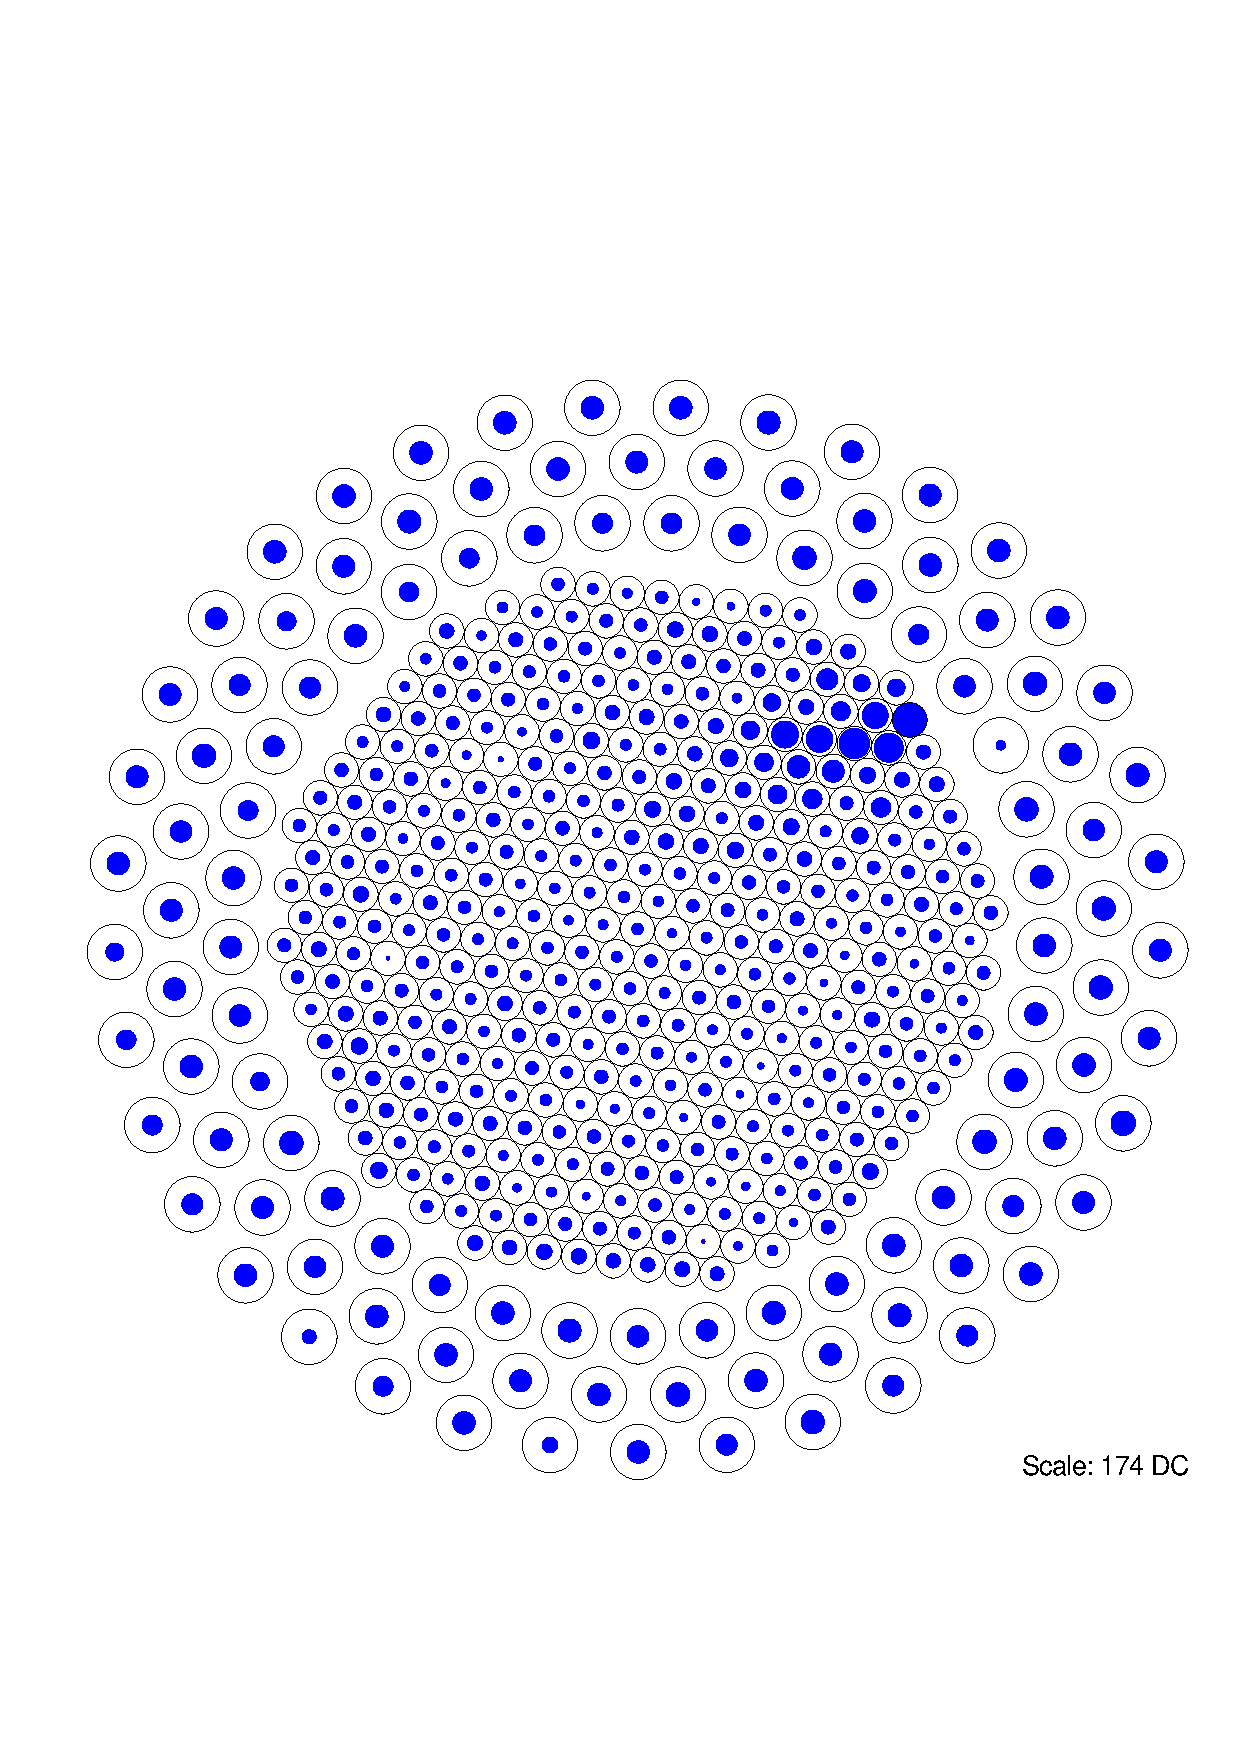
\includegraphics[draft=false]{plots/chap-analysis/gt023886_ev2652_raw.pdf}}%
\resizebox*{!}{\textheight}{\includegraphics[draft=false]{plots/chap-analysis/gt023886_ev2652_ped.pdf}}}}

\centerline{\resizebox{\textwidth}{!}{\resizebox*{!}{\textheight}{\includegraphics[draft=false]{plots/chap-analysis/gt023886_ev2652_gain.pdf}}%
\resizebox*{!}{\textheight}{\includegraphics[draft=false]{plots/chap-analysis/gt023886_ev2652_clean.pdf}}}}
\caption{\label{FIG::ANALYSIS::CONDITIONING} A typical event 
after each stage of image conditioning. (Top left) Raw ADC values. (Top
right) After subtraction of injected pedestals. (Bottom Left) After
gain equalization. (Bottom right) After cleaning.}
\end{figure}

\subsection{Pedestal Removal}
\label{SUBSEC::ANALYSIS::PEDESTAL}

The signal chain between the photo-tubes and ADCs is AC coupled at
the amplifier to remove any steady current associated with the
night-sky background and with any dark currents present in the PMT. To
allow negative fluctuations from the mean night-sky background to be
measured, a small biasing current is artificially injected into the
ADCs in order to yield a positive output for the largest reasonable
negative fluctuation, integrated over the 20\,ns ADC gate. This small
biasing current, dubbed the ``pedestal'', is set large enough to
accommodate a 4-5$\sigma$ negative fluctuation (with a typical, dark
sky, night-sky background rate) by adjusting a trim-potentiometer on
the ADC board. Typically the RMS fluctuations due to the night-sky
background are $\sim4-5$ digital counts (DC) when integrated by the
ADCs, so a bias current giving an integrated signal of $\sim20-25$\,DC
is chosen. The pedestal currents must be subtracted from the ADC
signals during the analysis to result in a mean of zero for each
channel when no signal is present.

In addition to the normal triggering requirement described in
section~\ref{SEC::TECHNIQUE::ELECTRONICS}, an artificial trigger is
generated from the 1\,Hz signal of the master GPS clock. This causes
events, which are flagged as special ``pedestal events'' in the data
stream, to be recorded in the absence of an air-shower. These events
record the zero-level point of each ADC in the presence of any
night-sky background and the injected pedestal current.

To estimate the level of the integrated pedestal current present in
each channel, these events are accumulated over the course of
observations (typically 1600 events in a 28\,minute scan), and the
mean recorded signal in each channel and its variance are
calculated. The mean value corresponds to the pedestal current
integrated over the gate time, expressed in DC. The variance gives
the mean-squared fluctuations in the night-sky background level
integrated in the gate, expressed in DC.

For all air-shower triggered events, the value of the pedestal is
subtracted from the signal to give the amount of charge recorded in
each channel, expressed in DC.

\subsection{Gain Equalization}
\label{SUBSEC::ANALYSIS::GAIN}

At the beginning of every night of observations, a calibration of the
relative gain of each channel across the camera is performed. By
illuminating the camera uniformly with the flashes from a fast
nitrogen arc lamp and recording the results, an estimate of the
relative gain in each channel is calculated. The N$_2$ lamp, which has
been demonstrated to illuminate the camera uniformly
\citep{REF::SCHROEDTER::2002PRIVATE}, produces fast $\sim$35\,ns
flashes at a rate of $\sim$750\,Hz. Neutral density filters are used
to attenuate the flashes so that they produce a manageable signal in
the ADCs ($\sim$700\,DC from the 10-bit maximum readout).

For any nitrogen arc flash, the signal in each channel\footnote{In
this chapter, the channel number is referred to by the index
$\alpha$}, $s^{(\alpha)}$, is given by the product of the number of
photons which strike the photo-cathode, $n_{ph}^{(\alpha)}$, the
efficiency of the PMT at collecting photons, $\eta^{(\alpha)}$, and
the gain of the channel, $g^{(\alpha)}$. The efficiency factor,
$\eta^{\alpha}$, accounts for the efficiency of the photo-cathode at
converting photons to photo-electrons and for the efficiency of tube
at collecting the photo-electrons. This efficiency depends, to some
extent, on the voltage across the tube (in particular the voltage
across the first dynode). It is convenient to introduce an overall gain
factor, $G$, to account for the average PMT gain, amplifier gains,
cable losses, ADC conversion factor and average PMT efficiency across
the camera. $G$ can be selected such that the mean of
$g^{(\alpha)}\eta^{(\alpha)}$ is unity.  The signal can therefore be
written,
\[s^{(\alpha)} = G\,g^{(\alpha)}\,\eta^{(\alpha)}\,n_{ph}^{(\alpha)}.\]

To flat-field the camera, i.e.\ to account for the different gains and
efficiencies across the camera, the factor
$g^{(\alpha)}\eta^{(\alpha)}$, must be calculated for each
channel. The efficiency factor is often incorporated into
$g^{(\alpha)}$ at this point, but will be kept in the calculations
below. The factor $g^{(\alpha)}\eta^{(\alpha)}$ is referred to
as the ``relative gain'' of the channel.

Since the mean relative gain is chosen to be unity (i.e.\ by choice of G),
the mean signal recorded for any nitrogen flash can be written,
\[\langle s^{(\alpha)}\rangle_\alpha = G\,\langle g^{(\alpha)}\eta^{(\alpha)}\,n_{ph}^{(\alpha)}\rangle_\alpha = G\,\langle g^{(\alpha)}\eta^{(\alpha)}\rangle_\alpha\,\langle n_{ph}^{(\alpha)}\rangle_\alpha = G\,\langle n_{ph}^{(\alpha)}\rangle_\alpha,\]
where the mean, $\langle\cdot\rangle_\alpha$, is shown explicitly to
be taken over all the channels. The signal in each channel can be
written relative to the mean as,
\[s^{(\alpha)}/\langle s^{(\alpha)}\rangle_\alpha =
g^{(\alpha)}\eta^{(\alpha)}\,n^{(\alpha)}/\langle n^{(\alpha)}\rangle_\alpha,\]
where the explicit label on $n_{ph}$ has been dropped. Accumulating a
large number of nitrogen flashes (labeled below by the index $i$) and
averaging over them for each channel gives the relative gain,
\[\left\langle\frac{s^{(\alpha)}_i}{\langle s^{(\alpha)}_i\rangle_\alpha}\right\rangle_i\ = 
g^{(\alpha)}\eta^{(\alpha)}\,\left\langle \frac{n^{(\alpha)}_i}{\langle n^{(\alpha)}_i\rangle_\alpha}\right\rangle_i\ =  
g^{(\alpha)}\eta^{(\alpha)}\,\frac{\langle n^{(\alpha)}_i\rangle_i}{\langle\,\langle n^{(\alpha)}_i\rangle_\alpha\,\rangle_i} =
g^{(\alpha)}\eta^{(\alpha)}\,\frac{\langle n\rangle}{\langle n\rangle} = g^{(\alpha)}\eta^{(\alpha)}.\]

These relative gain estimates are used to scale the signals in each
channel for every scan taken during the night.

In practice, gains calculated using this method suffer from a number
of deficiencies arising from the fact that the average profile of the
nitrogen arc pulses is different from that of \Cerenkov pulses from
air showers; the duration of the N$_2$ pulses are significantly longer
with a longer decay time. The ADC integration gate is chosen to
accommodate all but the largest \Cerenkov pulses with a minimum of
sky-noise. Because of their fast fall-off, small differences (1-2\,ns)
in the start time or duration of the gate signal between ADC modules
does not significantly effect the signal recorded from \Cerenkov
pulses, but does have a larger effect on N$_2$ pulses which have not
decayed by the end of the integration time. Another approach to gains
calculation is to measure the spectrum of the cosmic-ray background
during the course of a night. Over the course of a few hours of
observations, sufficient cosmic-ray background events can be collected
to allow differences in the spectrum in each channel, due only to a
difference in the gain of each channel, to be detected. Since the
background events have the same time profile as the \Gray events of
interest, this method does not suffer from the systematic differences
as the nitrogen pulser method. The nitrogen method, which is the
standard method of gain equalization used when analyzing Whipple data,
has been used in this work.

\subsection{Channel Sanity Checking}
\label{SUBSEC::ANALYSIS::SANITY}

In order to minimize the effects of bright stars in or adjoining the
field of view, noisy channels and PMTs whose gain is set very high or
low, two simple sanity checks are applied to the data. Channels whose
RMS pedestal fluctuations are too high, or too low with respect to the
median pedestal fluctuation across all the channels in the camera are
``turned off in software'', i.e.\ their signals are disregarded during
image parameterization in all events in both the \On\ and \Off\ data
scans.  The requirement for a channel to be included in the
parameterization is that, $0.6\,\mathrm{med}(\sigma^{(\alpha)}) <
\sigma^{(\alpha)} < 1.5\,\mathrm{med}(\sigma^{(\alpha)})$. Additionally, 
channels whose relative gains are very different from the median gain
across the camera, i.e.\ those which do not satisfy the following
$0.1\,\mathrm{med}(g^{(\alpha)}\eta^{(\alpha)}) < 
g^{(\alpha)}\eta^{(\alpha)} < 
5.0\,\mathrm{med}(g^{(\alpha)}\eta^{(\alpha)})$, are also excluded.

\subsection{Image Cleaning}
\label{SUBSEC::ANALYSIS::CLEANING}

The parameterization technique employed, based on the principal
moments of the light distribution in the image, is sensitive to
fluctuations of the night-sky background. In particular, the second
order moments of the distribution will be skewed by channels with
large night-sky induced signals which lie far from the image of the
shower. In order to minimize the effects of these ``outliers'' a
cleaning procedure is applied to the image
\citep{REF::FEGAN::SSR1996}. Those channels which have a signal
larger than a threshold, $n_{img}$, times the RMS night-sky
fluctuation in that channel are denoted as ``image channels''. Those
with a signal greater than a different threshold, $n_{bnd}$, times the
RMS night-sky fluctuation and, in addition, are located adjacent to an
``image channel'' are denoted ``boundary channels''. All channels in
the image that are not in either of these categories are discarded. In
choosing the thresholds a compromise must be reached between
eliminating the noise in the image and keeping channels with a small
signal which are part of the air-shower image. This is particularly
important to ensure good differentiation between compact \Grayc-like
events and broad cosmic-ray-like events. For this work, the values of
$n_{img}$=4.25 and $n_{bnd}$=2.25 are chosen. These values are
standard for the analysis of Whipple 10\,m data during this period.

\subsection{Noise Padding}
\label{SUBSEC::ANALYSIS::PADDING}

As described above, when operating in \Pairs\ mode, two 28\,minute
scans are taken, each covering the same range in azimuth and
elevation. This ensures that local contributions to the background
rate, e.g.\ due to light pollution from the neighboring cities of
Tucson and Nogales, are introduced equally to both scans. Significant
differences can still arise due to non-local differences between the
\On\ and \Off\ scans, such as the presence of bright stars or the
Galactic Plane in either of the fields. For candidates that lie near
to the Galactic Plane, the field of the \Off\ scan will not, in
general, also lie on the Plane. The night-sky background flux varies
by a factor of two, from
${\langle}NSB_{\mathrm{flux}}\rangle$\,$\approx$\,2--4$\times$10$^{12}$\,s$^{-1}$m$^{-2}$sr$^{-1}$,
between locations away from, and on, the Galactic Plane. There are two
major effects of such brightness differences, the first on the image
cleaning algorithm described above, the second on the hardware
trigger.

As described above, image cleaning discards channels whose signal to
noise ratio is smaller than a certain threshold. An air-shower signal
recorded in a channel which has a larger noise component will have a
smaller S/N ratio and will therefore be more likely to be
discarded. This is not a problem for channels in the core of a bright
shower, but weak signals from the periphery of a shower will tend to
be preferentially discarded by the cleaning algorithm in a region with
a bright night-sky background contribution. This has the effect of
making the shower image tend to appear smaller. Since the data
selection procedure (described below) is based on eliminating all but
the most compact images, systematic differences will arise due to
cleaning between \On\ and \Off\ scans, where large night-sky
differences exist. To compensate for this, artificially generated
Gaussian noise is added to equalize the noise between the two scans,
in a process known as ``software padding''.

For each channel, the noise in the \On\ and
\Off\ fields ($\sigma_\mathrm{On}^{(\alpha)}$ and
$\sigma_\mathrm{Off}^{(\alpha)}$) are calculated from pedestal events
as described above. In general, for each channel, one field will have
more noise present than the other, say
$\sigma_\mathrm{On}^{(\alpha)}>\sigma_\mathrm{Off}^{(\alpha)}$
($\sigma_\mathrm{On}^{(\alpha)}<\sigma_\mathrm{Off}^{(\alpha)}$). To
compensate, for this channel, Gaussian noise is added to all events of
the \Off\ (\On) scan. Since the noise variance adds in quadrature, the
level of padding noise added is given by
$\Delta\sigma_\mathrm{Pad}^{(\alpha)}=\sqrt{|\sigma_\mathrm{On}^{(\alpha)\,2}-\sigma_\mathrm{Off}^{(\alpha)\,2}|}$. For
well matched \On\ and \Off\ fields, small amounts of noise will be
added to both fields. For scans where there is a large systematic
difference, one field will have more noise added to it than the
other. During cleaning, the S/N ratio of channels in both the \On\ and
\Off\ scans is calculated using the common value of
$\sigma_\mathrm{Pad}^{(\alpha)}=\max(\sigma_\mathrm{On}^{(\alpha)},\,\sigma_\mathrm{Off}^{(\alpha)})$
for the noise level.

The padding technique, introduced in \citet{REF::CAWLEY::1993CALGARY},
has been employed successfully for a decade when analyzing Whipple
data. Previous generations of the Whipple instrument were fitted with
1\,inch diameter photo-tubes whereas the high-resolution camera, with
which the data in this survey was collected, employs 0.5\,inch
PMTs. This corresponds to a decrease in the collected night-sky
background by a factor of four, from $\sim8$ photo-electrons (PE) in a
20\,ns gate to $\sim1.8$\,PE. With previous cameras it was assumed
that this background could be approximated by a Gaussian distribution;
this assumption is no longer valid, except in the brightest regions of
the sky. Therefore, it could be argued that padding should be
performed with a non-Gaussian noise distribution. 
Table~\ref{TABLE::ANALYSIS::PADDING} shows the measured width of the
noise distribution for three channels selected from an
\Pairs\ mode observation before and after padding. The channels were
chosen to have the smallest and largest differences in noise between
the \On\ and \Off\ scans. An intermediate value was also chosen,
corresponding to the channel with the largest difference that would
have passed the sanity check described above. It can be seen from the
table that the difference between the noise levels after padding is
not large in any of the cases, the maximum being 4\%. Any improvement
to be gained from padding with a more realistic modeling of the noise
distribution is expected to be small and was not undertaken for the
data analyzed in this work.

\begin{table}[t]
\caption{\label{TABLE::ANALYSIS::PADDING} Difference between 
noise levels for three channels, before and after software noise padding.}
\centerline{\begin{tabular}{llllll}\hline
& \multicolumn{2}{l}{Before Padding} & & \multicolumn{2}{l}{After Padding} \\
\raisebox{1.5ex}[0pt]{Relative $\sigma_\mathrm{Pad}^{(\alpha)}$} & 
$\sigma_\mathrm{On}^{(\alpha)}$ & $\sigma_\mathrm{Off}^{(\alpha)}$ &
\raisebox{1.5ex}[0pt]{$\sigma_\mathrm{Pad}^{(\alpha)}$} & 
$\sigma_\mathrm{On}^{(\alpha)}$ & $\sigma_\mathrm{Off}^{(\alpha)}$ \\\hline
Smallest & 4.21\,DC & 4.03\,DC & 1.21\,DC & 4.21\,DC & 4.37\,DC \\ % 3.72\%
Intermediate$^1$ & 6.36\,DC & 4.43\,DC & 4.56\,DC & 6.36\,DC & 6.40\,DC \\ % 0.6\%
Largest & 9.03\,DC & 4.34\,DC & 7.92\,DC & 9.03\,DC & 8.69\,DC \\\hline % 3.83\% 
\end{tabular}}

\vspace{1.5ex}\centerline{\begin{minipage}{0.9\textwidth}
$^1$ Intermediate value corresponds to channel with largest night-sky
noise which would survive sanity check, as described above.
\end{minipage}}
\end{table}

Finally, as mentioned above, differences in the background sky
brightness will also influence the triggering rate of the
instrument. Individual stars in the field of view can usually effect a
number of neighboring channels and essentially decrease the triggering
threshold in one small region of the camera. This star-induced effect
is not serious as the ``hot'' channels will usually be eliminated from
the analysis by the sanity checks. More troublesome is a large scale
brightness difference between the \On\ and \Off\ fields which can
decrease the effective triggering threshold across the camera causing
more events to be recorded in the brighter field. It is possible to
compensate for this effect during analysis by imposing a higher
triggering threshold. Another approach which can be adopted is to scale
the number of counts recorded in the calculation of the background
estimate.

\section{Parameterization}
\label{SEC::ANALYSIS::PARAMETERIZATION}

Events are parameterized by the moments of the light distribution in
the image. The zeroth, first and second moments describe the total
light in the image, the ``center of mass'' of the light distribution
in the camera and the length, width and orientation of the
distribution.  Given that each channel is located at coordinates
$x^{(\alpha)}_i$ in the camera and records a signal $s^{(\alpha)}$,
the first three orders of moments are,
\begin{eqnarray*}
S = X^{(0)} & = & \sum_\alpha s^{(\alpha)} \\
(x_c, y_c) = \bar{x}_i = X^{(1)}_i & = & \sum_\alpha s^{(\alpha)}x^{(\alpha)}_i / S \\
\sigma_{ij} = X^{(2)}_{ij} & = & \sum_\alpha 
s^{(\alpha)}(x^{(\alpha)}_i-\bar{x}_i)(x^{(\alpha)}_j-\bar{x}_j)/S
\end{eqnarray*}

It is usual to refer to the parameter S as the \textit{size} of the
image and to define a parameter describing the distance between the
center of the camera and the image centroid as
$distance=\sqrt{x_c^2+y_c^2}$. The \textit{length},
\textit{width} and \textit{orientation} of the image are derived by 
diagonalizing the matrix of second order moments, i.e.\ by finding 
the value of $\theta$ such that,
\[\left(\begin{array}{cc} \sigma_{11} & \sigma_{12} \\ 
\sigma_{21} & \sigma_{22} \end{array} \right) =
\left(\begin{array}{cc} \cos\theta & \sin\theta \\ 
-\sin\theta & \cos\theta \end{array} \right) 
\left(\begin{array}{cc} length^2 & 0 \\ 
0 & width^2 \end{array} \right) 
\left(\begin{array}{cc} \cos\theta & -\sin\theta \\ 
\sin\theta & \cos\theta \end{array} \right).\]

\begin{figure}[t]
\centerline{\resizebox{\textwidth}{!}{\resizebox*{!}{\textheight}{\includegraphics[draft=false]{plots/chap-analysis/gt023886_ev2652_param.pdf}}%
\resizebox*{!}{\textheight}{\includegraphics[draft=false]{plots/chap-analysis/param.pdf}}}}
\caption{\label{FIG::ANALYSIS::PARAM} (left) Sample image 
taken with the high resolution camera, after image conditioning, with 
image axis and second order moments indicated. (right) Illustration 
of image parameters.}
\end{figure}

From these moments a number of useful parameters are calculated
\citep[see appendices of][]{REF::REYNOLDS::APJ1993}. In particular,
the \textit{alpha} parameter is important to the analysis of data from
a candidate point-source object at the center of the field of view. As
illustrated in figure~\ref{FIG::ANALYSIS::PARAM},
\textit{alpha} describes the orientation of the shower image with
respect to the line joining the source location and the centroid of
the image distribution. Images with a small value of \textit{alpha}
(usually $\alpha<15^\circ$) are considered to be consistent with
having originated from the source location; those with a large value of
\textit{alpha} are not. In a standard point source analysis, a
histogram is made of the alpha parameter for all events which pass the
data selection criteria. An excess of events with small \textit{alpha}
is indicative of a source at the center of the field of view.

\section{Data Selection}
\label{SEC::ANALYSIS::DATASELECTION}

Data selection is based on strict cuts of the parameter values
described above. Cuts can be considered as belonging to two
categories.  The first set is used to address undesirable effects that
arise due to the instrument itself, the second to preferentially
retain \Gray events while eliminating the background. The values that
parameters must have to survive the cuts are chosen by optimizing the
response of the system to a known \Gray source, usually the steady
flux from the Crab Nebula. The standard set of cuts used on Whipple
data is known as ``Supercuts''. Since ``Supercuts'' were optimized for
point source detection, a new set of cuts were developed for this
work, termed ``Loosercuts''. They were chosen to accept more events,
relying on the 2-dimensional reconstruction to increase the S/N
ratio. Additionally a set of cuts optimized to keep only events with
energy $>\sim$1\,TeV has been developed.

Cuts in the first category are largely the same for both sets. They
consist of three cuts, known as \textit{trigger}, \textit{distance}
and \textit{size}. The \textit{trigger} cut reduces the effects of
unevenness in the hardware trigger by requiring that the two largest
signals recorded in the event are greater than 30\,DC. The
\textit{distance} cut, which eliminates those events occuring at the
edge of the camera and which may be truncated, is listed in
table~\ref{TABLE::ANALYSIS::CUTS}. The \textit{size} cut, a cut on the
total signal recorded in the image, is not applied in Supercuts, but
can be used to adjust the peak response energy (P.R.E.) of the
instrument. For example a cut requiring $size>1500$\,DC gives a
P.R.E.\ of $\sim$1\,TeV.

The second category of cuts are based largely on the shape
(\textit{length} and \textit{width}) of the image. The shape cuts are
listed in table~\ref{TABLE::ANALYSIS::CUTS}. The bulk of the
background is eliminated by the strict \textit{width} cut which is
optimized to keep the compact \Gray events while eliminating the
broader cosmic-ray images.  Additionally a cut on the ratio of the
length of the image to the amount of light present,
$length/size<0.0004$, is used to eliminate a large fraction of the
background muon images.

\begin{table}[t]
\caption{\label{TABLE::ANALYSIS::CUTS} Data selection cuts 
used in this work.}
\centerline{\begin{tabular}{lllll}\hline
Parameter & \multicolumn{2}{l}{Supercuts} & Loosercuts & 1\,TeV Loosercuts \\\hline
\textit{distance} & $>$\,0.40$^\circ$ & $<$\,1.00$^\circ$ & $<$\,1.00$^\circ$ & $<$\,1.00$^\circ$ \\
\textit{length}   & $>$\,0.05$^\circ$ & $<$\,0.12$^\circ$ & $<$\,0.14$^\circ$ & $<$\,0.14$^\circ$ \\
\textit{width}    & $>$\,0.13$^\circ$ & $<$\,0.25$^\circ$ & $<$\,0.35$^\circ$ & $<$\,0.35$^\circ$ \\
\textit{size}     & n/a & n/a & n/a & $>$1500\,DC \\\hline
\end{tabular}}
\end{table}

\section{2D Analysis technique}
\label{SEC::ANALYSIS::2D}

For extended sources or sources where the source location is not well
determined, it is essential to reconstruct the arrival direction of
the primary. This can be done naturally using systems of telescopes
observing the shower from a number of different positions on the
ground, as described in chapter~\ref{CHAP::VERITAS}. For a single
telescope, the arrival direction must be inferred from the
\textit{shape} and \textit{orientation} of the single observed
image.
% A number of two dimensional reconstruction methods have been
%developed by others and employed successfully. 
The approach taken here is based on \citet{REF::LESSARD::2001APP}.

Although the shower processes are stochastic in nature, there is a
statistical relationship between the parameters of the recorded image
and a set of parameters, denoted $\Theta$, which describe the energy
and path of the incident {\Grayc}, \mbox{$\Theta=\{E, x_0, y_0,
b, \psi\}$}. The parameter $E$ refers to the energy of the primary
{\Grayc}. The pair, $(x_0, y_0)$ denote the direction of propagation of 
the \Gray with respect to the axis of the telescope, i.e.\ the
location in the field of view of the of the source of the {\Grayc}. The
final two parameters, $(b, \psi)$, denote the point of closest
approach of the propagation of the primary \Gray to the camera; $b$ is
conventionally called the impact parameter, $\psi$ denotes the
direction to the point of closest approach.

The following relationships exist, in a statistical sense, between the
image parameters and the shower parameters
\begin{eqnarray}\label{EQN::ANALYSIS::IMAGEPARAM}
length & = & length(E, b) \\
width & = & width(E, b) \\
size & = & size(E, b) \\
(x_c, y_c) & = & (\;x_c(E, x_0, y_0, b, \psi), y_c(E, x_0, y_0, b, \psi)\;) \\
\theta & = & \theta(x_0, y_0, \psi) \label{EQN::ANALYSIS::IMAGEPARAM::FINAL}
\end{eqnarray}
where any contribution to the parameters due to optical aberrations
and clipping of the image due to the finite size of the camera have
been ignored. The requirement of two-dimensional reconstruction is to
find a relationship between the image parameters and the direction of
propagation of the \Gray, i.e.\ to find,
\begin{eqnarray*}
x_0 & = & x_0(size, length, width, x_c, y_c) \\
y_0 & = & y_0(size, length, width, x_c, y_c)
\end{eqnarray*}
In practice, it is more convenient to estimate the arrival direction
of the primary with respect to the image centroid, $\Delta x=x_c-x_0,
\Delta y=y_c-y_0$. As illustrated in
figure~\ref{FIG::ANALYSIS::2DPARAM}, the \Gray source location lies
along the shower axis (disregarding errors in axis reconstruction),
whose direction in the camera is described by $\theta$. It is
convenient to define a new shower parameter, $disp$, as the distance
between the image centroid and the source location, by $\Delta x=disp
\cos\theta,
\Delta y=disp \sin\theta$. In general, $disp=disp(E, b)$, i.e.\ is
dependent only on the energy and impact parameter of the primary. If
the relationships,
equations~\ref{EQN::ANALYSIS::IMAGEPARAM}--\ref{EQN::ANALYSIS::IMAGEPARAM::FINAL},
are valid, then $disp$ can be written in terms of the shower image
parameters, $disp=disp(size, length, width).$

\begin{figure}[t]
\centerline{\resizebox{\textwidth}{!}{\resizebox*{!}{\textheight}{\includegraphics[draft=false]{plots/chap-analysis/twodim.pdf}}\hspace*{1cm}%
\resizebox*{!}{\textheight}{\includegraphics[draft=false]{plots/chap-analysis/threedim.pdf}}}}
\caption{\label{FIG::ANALYSIS::2DPARAM} Illustration of 
shower parameter $disp$ in the field of view of camera (left) and from 
perspective of the shower in the atmosphere (right).}
\end{figure}

\enlargethispage{12pt}
When the shower impact location is zero, there is no preferred
direction in the shower image, i.e.\ $length=width$, and the
image centroid and source location coincide, i.e.\ $disp=0$. This
suggests that $disp$ should be expanded in terms of the shower 
ellipticity, $\epsilon=1-width/length$,
\[disp = a_1(size,length)\times \epsilon + a_2(size,length)\times \epsilon^2 + \cdots.\]
Simulations, detailed in appendix~\ref{APP::ELLIPT}, which assume that
the dependence of $a_i$ on $length$ is of secondary importance,
indicate that the quadratic term, $a_2$, is unnecessary and the $a_1$
can be reasonably approximated as
\[a_1 = 1.36^\circ + 0.14^\circ\log(size/1622\,\mathrm{DC}).\]

For this work, a simpler assumption was made, following
\citet{REF::LESSARD::2001APP}. The dependence on \textit{size} was
neglected completely and the displacement between source location and
image centroid was assumed to be given simply as the product of a
constant, $\xi$ and the ellipticity,
\begin{equation}
\label{EQN::ANALYSIS::DISP}disp = \xi \times \left(1-\frac{width}{length}\right)
\end{equation}
This approach is justified empirically using observations of the Crab
Nebula, deliberately offset from the center of the camera by various
degrees, as detailed below.

A sky map is produced by constructing a 2-dimensional histogram
of the reconstructed arrival direction with respect to the center of
the camera. Errors in reconstructing both the image axis and $disp$
are accounted for by convolving the final 2D map with a Gaussian
smoothing function
\(g(\vec{r};r_0)= \exp(-r^2/2r_0^2)\), where $r_0$ is a scaling parameter
chosen to maximize the significance of an excess. 
Appendix~\ref{APP::SMOOTHING} discusses the advantage of Gaussian 
smoothing over that of \citet{REF::LESSARD::2001APP}.

This method yields two possible arrival directions for each event,
each of which is on the major axis of the shower image, separated from
the centroid by the calculated parameter, $disp$.  In creating a 2D
map of the detected events, the origin of each event is assigned to
both possible directions in the hope that one will have an excess as
the event origins are superimposed.

Calculation of excess signal, significance and upper-limit maps
($S(\vec{r})$, $\sigma(\vec{r})$ and $UL(\vec{r})$ respectively) is
then done by convolving the \On\ and \Off\ counts with the smoothing
function $g(\vec{r})$ in the appropriate manner,
\begin{eqnarray}
S(\vec{r}) & = & \sum_{\vec{r'}}{[(ON(\vec{r'})-OFF(\vec{r'})]g(\vec{r'}-\vec{r})} \label{EQN::ANALYSIS::SMOOTHEXCESS}\\
\Delta S(\vec{r})^2 & = & \sum_{\vec{r'}}{[ON(\vec{r'})+OFF(\vec{r'})]g^2(\vec{r'}-\vec{r})} \label{EQN::ANALYSIS::SMOOTHDELTAEXCESS}
\end{eqnarray}
Then $\sigma(\vec{r})=S(\vec{r})/\Delta S(\vec{r})$ and $UL(\vec{r})$
is calculated from $S(\vec{r})$ and $\Delta S(\vec{r})$ by the method
of \citet{REF::HELENE::1983NIM}.

Calibration of the two dimensional analysis method was done using sets
of observations of the Crab Nebula, in which its location was
deliberately offset from the center of the field of view by various
degrees. Calculating the relative \Gray rate allows a model of the
detector response for off-axis and extended sources to be made.
Table~\ref{TABLE::ANALYSIS::2DOPTIMIZATION} lists the values of $\xi$
and $r_0$ found to be optimal. It also lists the rate of \Grays
detected from the Crab Nebula, normalized to 1.0 for the 2000-2001
season.

\begin{table}[t]
\caption{\label{TABLE::ANALYSIS::2DOPTIMIZATION} Optimized 
two-dimensional analysis parameters, calculated for observing seasons 
from 1999 to 2003.}
\centerline{\begin{tabular}{lllll}\hline
& 1999-2000 & 2000-2001 & 2001-2002 & 2002-2003 \\\hline
%\textbf{Loosercuts} & & & & \\
$\xi$ & 1.5$^\circ$ & 1.5$^\circ$ & 1.5$^\circ$ & 1.5$^\circ$ \\
r$_0$ & 0.175$^\circ$ & 0.175$^\circ$ & 0.175$^\circ$ & 0.175$^\circ$ \\
Relative Crab Rate & 0.86 & 1.00 & 0.91 & 0.80 \\\hline
%& & & & \\ \textbf{1\,TeV Loosercuts} & & & & \\
%$\xi$ & ZZZ & ZZZ & ZZZ & ZZZ \\
%r$_0$ & ZZZ & ZZZ & ZZZ & ZZZ \\
%Relative Crab Rate & ZZZ & ZZZ & ZZZ & ZZZ \\\hline
\end{tabular}}
\end{table}

\begin{figure}[p]
\begin{minipage}{0.33\textwidth}\centerline{On axis}\end{minipage}%
\begin{minipage}{0.33\textwidth}\centerline{0.3$^\circ$ off axis}\end{minipage}%
\begin{minipage}{0.33\textwidth}\centerline{1.3$^\circ$ off axis}\end{minipage}\\[0.5ex]
\centerline{{\resizebox*{0.33\textwidth}{!}{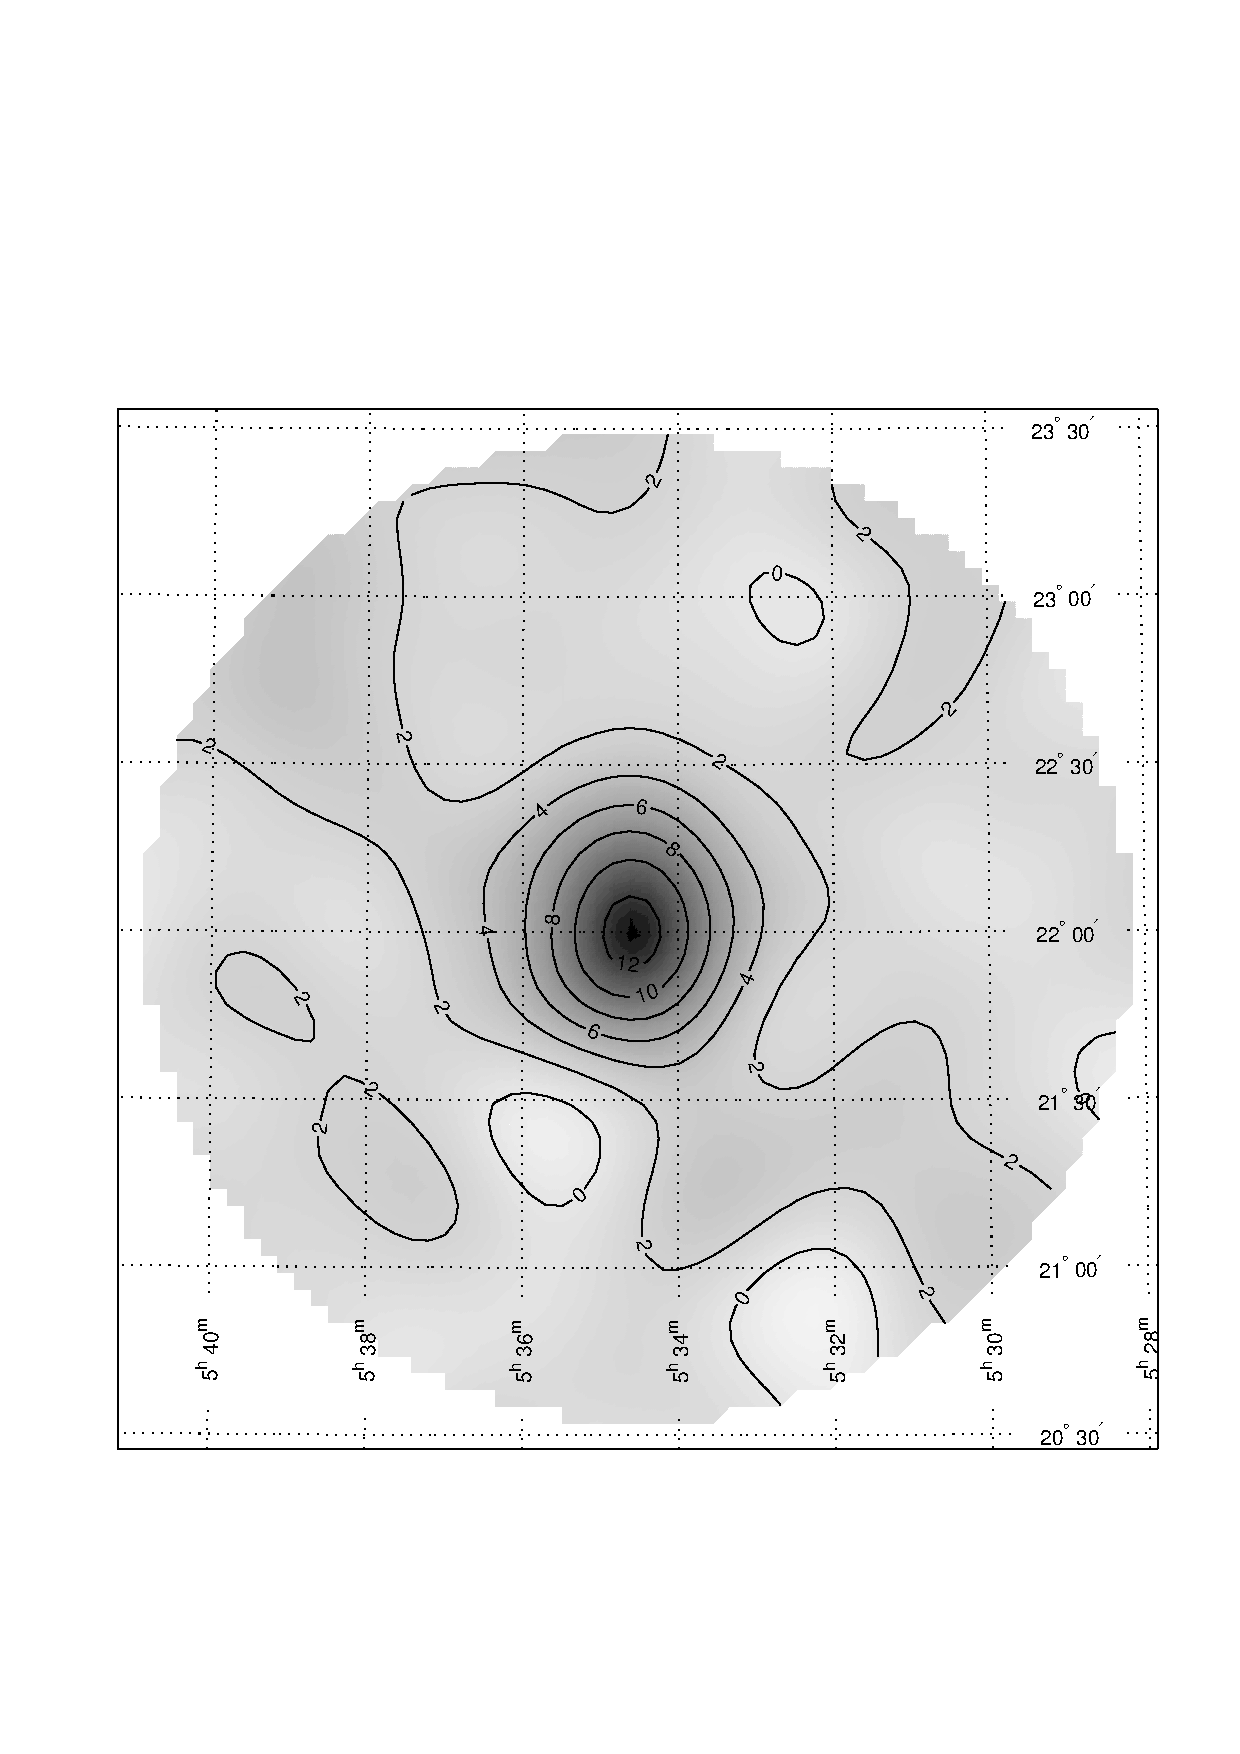
\includegraphics[draft=false]{plots/chap-analysis/crab_0_0_y0001_sig_bw.pdf}}%
\resizebox*{0.33\textwidth}{!}{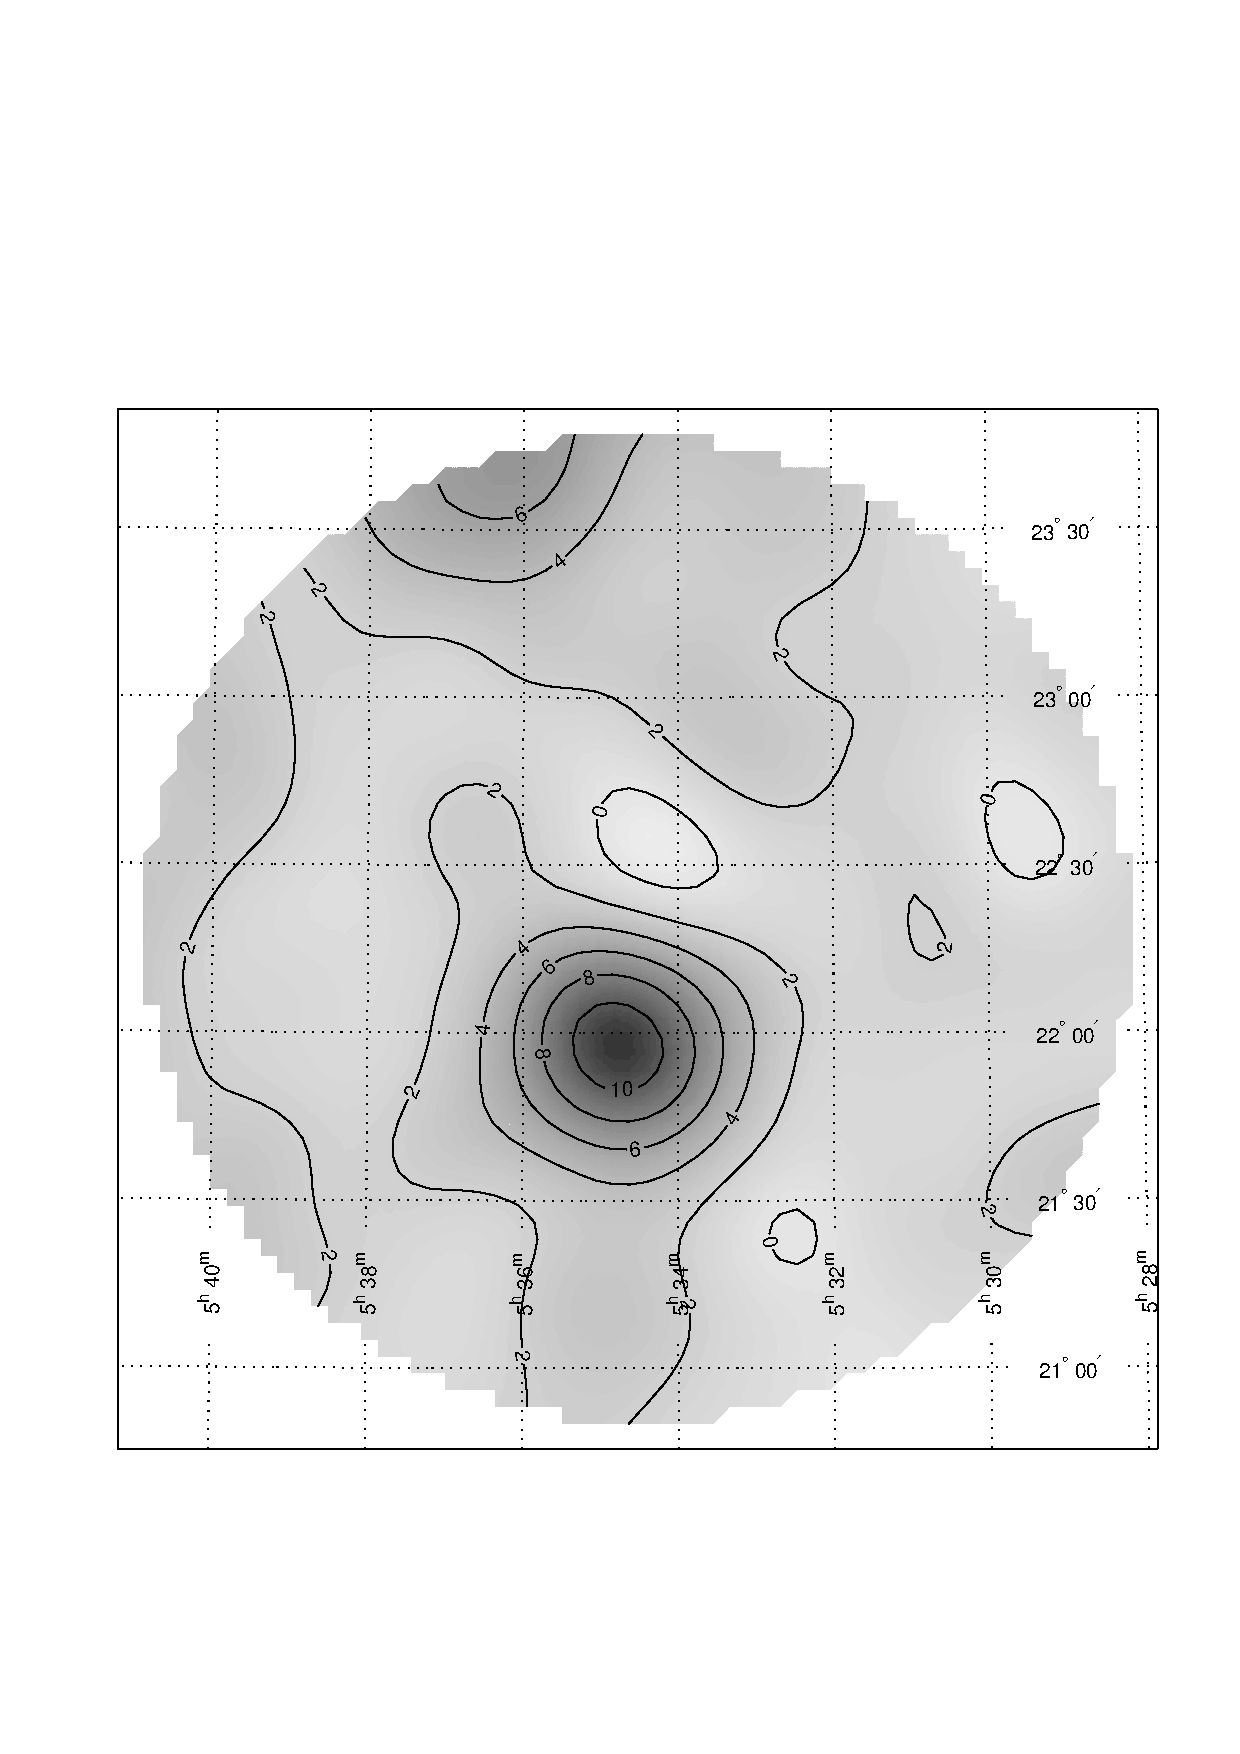
\includegraphics[draft=false]{plots/chap-analysis/crab_0_3_y0001_sig_bw.pdf}}%
\resizebox*{0.33\textwidth}{!}{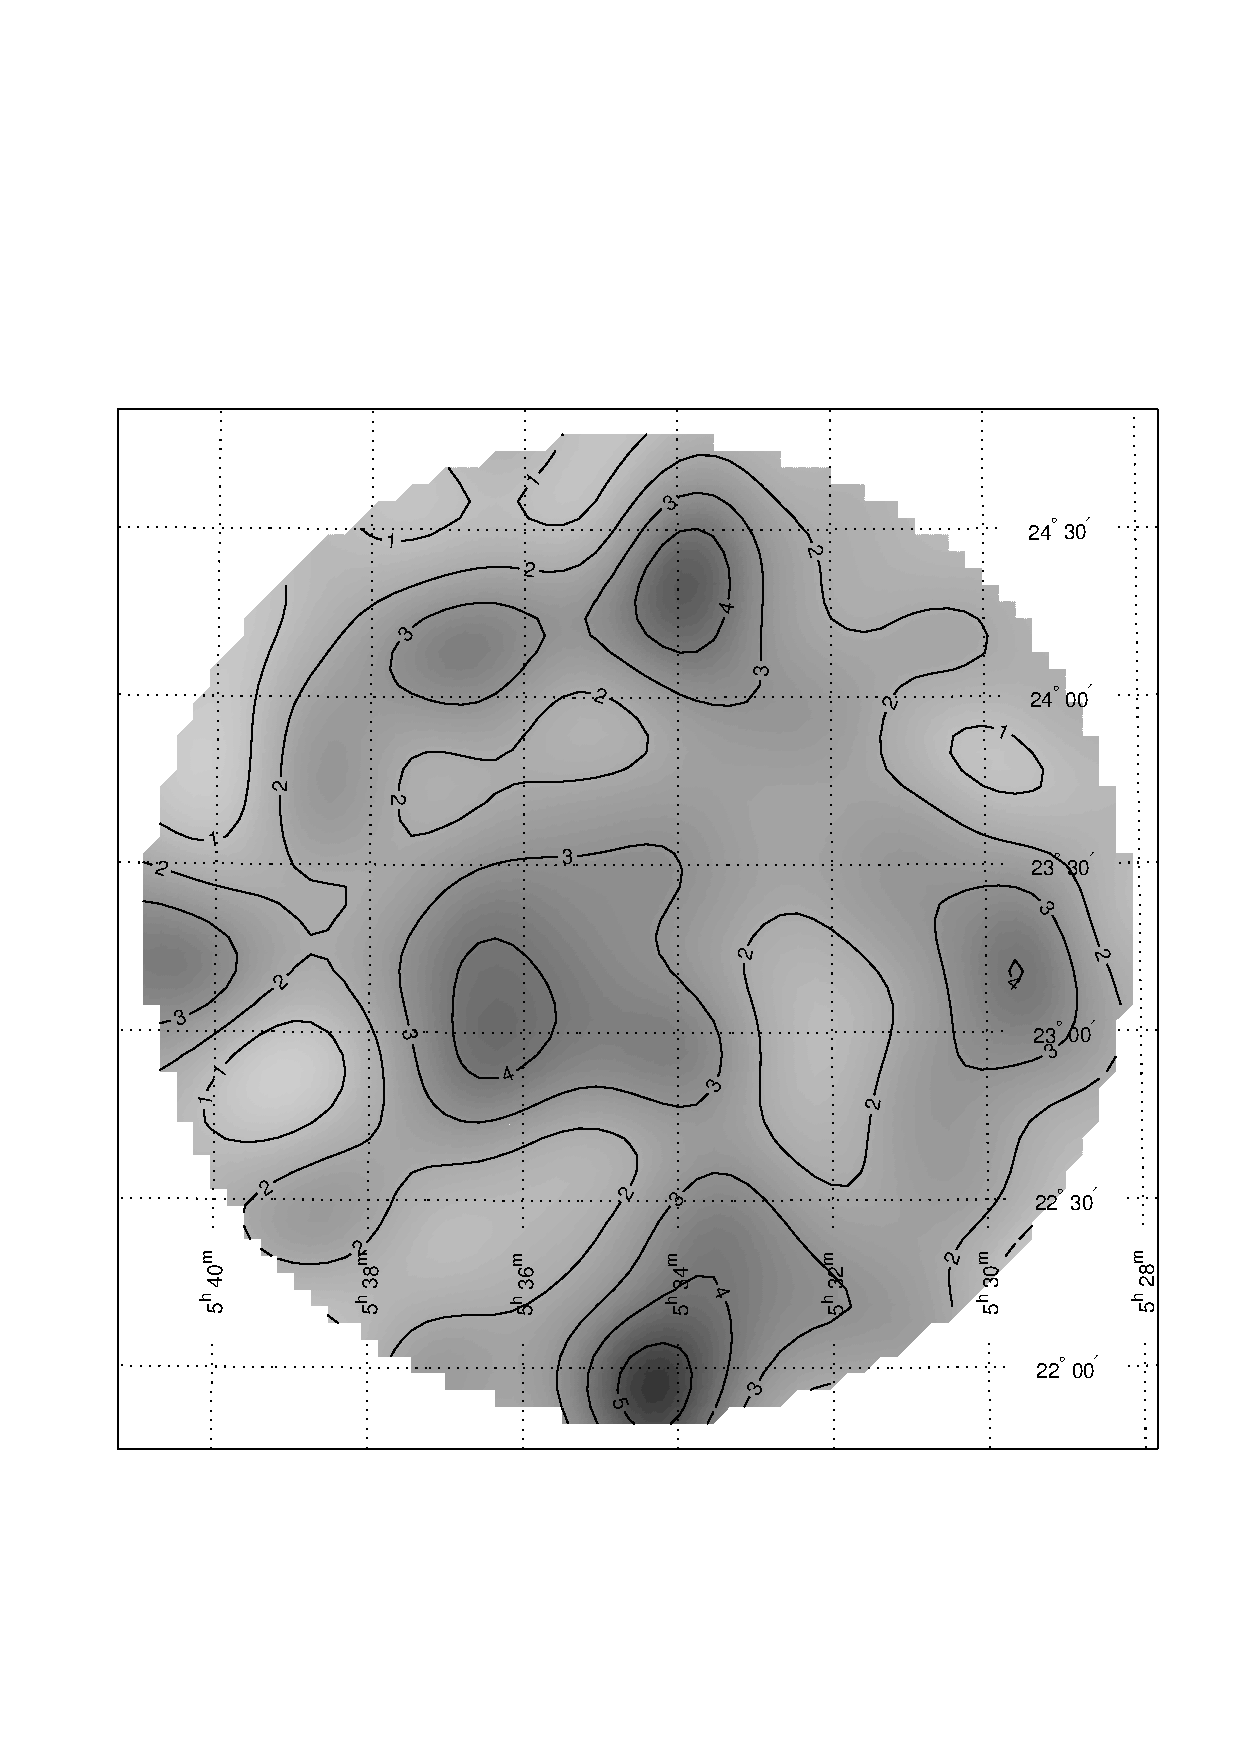
\includegraphics[draft=false]{plots/chap-analysis/crab_1_3_y0001_sig_bw.pdf}}}}
\caption{\label{FIG::ANALYSIS::2DSIGMA} Observations of the 
Crab Nebula, offset by varying amounts from the center of the field of 
view. The contours show detection significance. The observations at an 
offset of $1.3^\circ$ place the Crab outside of this.}
\end{figure}

Figure \ref{FIG::ANALYSIS::2DSIGMA} shows significance maps for the
Crab Nebula offset by three different amounts. In each of them the
Crab is clearly visible. At an offset of $0.3^\circ$ the \Gray
collection efficiency is $84$\% of what it is on axis.  At an offset
of $1.3^\circ$, with the source outside of the geometrical extent of
the camera, the efficiency is $30$\%. The significance map for this
data shows appreciable background contamination over the field due to
the simple reconstruction approach of assigning the arrival direction
of each photon to two points on the shower axis. More sophisticated
approaches can reduce such false sources
\citep{REF::LESSARD::2001APP}.

\begin{figure}[p]
\centerline{\resizebox*{\textwidth}{!}{\rotatebox{270}{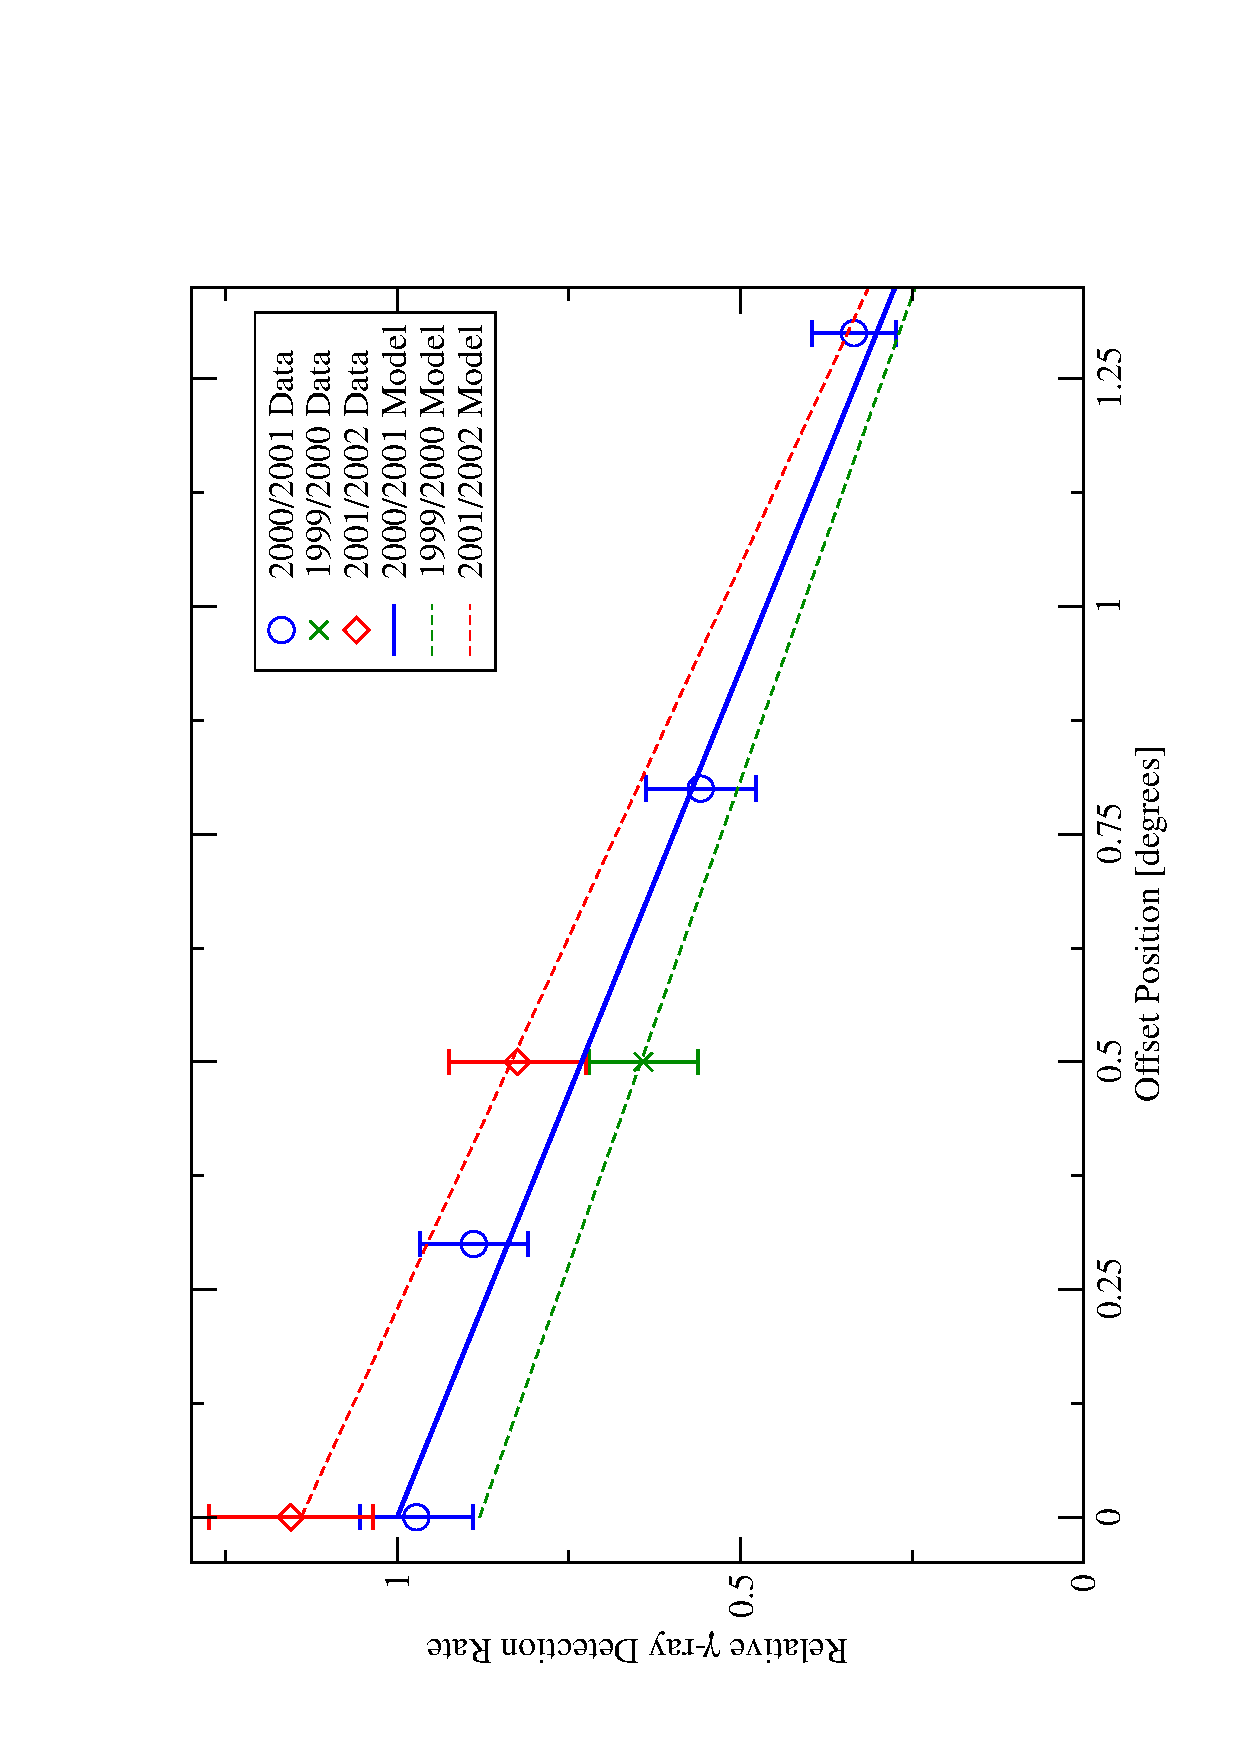
\includegraphics{plots/chap-analysis/rate_model.pdf}}}}
\caption{\label{FIG::ANALYSIS::2DRATE} Relative Crab detection rate as 
a function of source offset. The off-axis response can be fit by a 
straight line.}
\end{figure}

Figure \ref{FIG::ANALYSIS::2DRATE} shows the relative collecting
efficiency for offset sources. This curve is used to normalize
detected emission rates or upper limits to the Crab flux. 

\section{Significance of Observations}
\label{SEC::ANALYSIS::SIGNIFICANCE}

The calculated significance, $\sigma(\vec{r})$, described above,
corresponds to the confidence that the null hypothesis, i.e.\ that no
source is present at that point in the sky, is false. A large value of
significance can be thought of as giving a high confidence that a
source is present at the location. In the absence of any source,
$\sigma(\vec{r})$ should be distributed as Gaussian with unity width,
for any location in the field of view ($\vec{r}$) chosen a priori. To
ensure that the measurement of sigma is not biased, ``dark-field''
observations were analyzed. The analysis was applied to $240$
observations from 1999 to 2003 which were taken on regions of the sky
which are assumed to have no source present in them, i.e.\
observations on candidate point-source objects whose analysis did not
result in any significant excess. The significance of any excess (or
deficit) found in the center bin, $\sigma(\vec{0})$, of the sky map
from each of the observations is displayed in
figure~\ref{FIG::ANALYSIS::SIGMACENTER}.

\begin{figure}[p]
\centerline{\resizebox*{0.7\textwidth}{!}{\rotatebox{270}{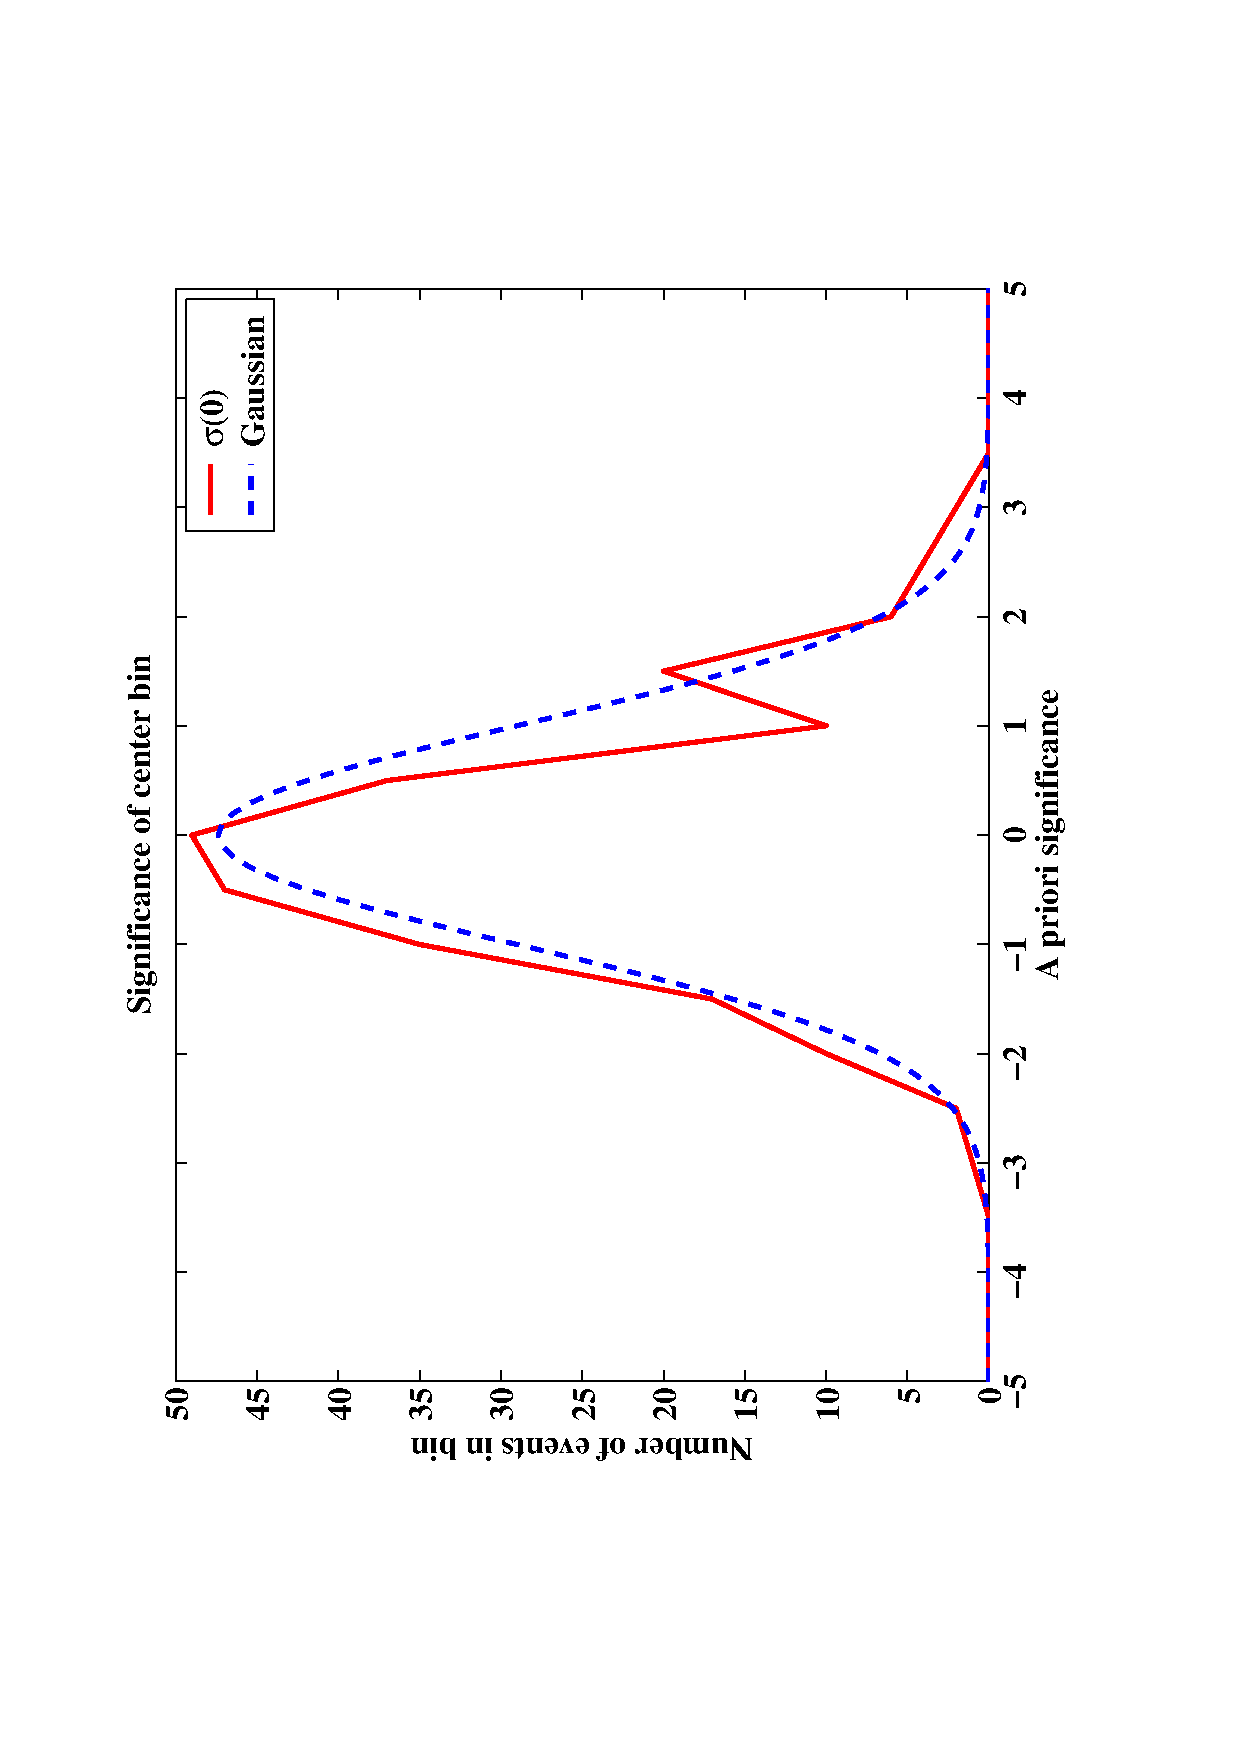
\includegraphics{plots/chap-analysis/sigma_center.pdf}}}}
\caption{\label{FIG::ANALYSIS::SIGMACENTER} Significance of 
excess (deficit) in counts in center bin of $240$ background observations. 
A Gaussian function of unity width, integrated over the binning size, 
is also shown.}
\end{figure}

\begin{figure}[p]
\centerline{\resizebox*{0.7\textwidth}{!}{\rotatebox{270}{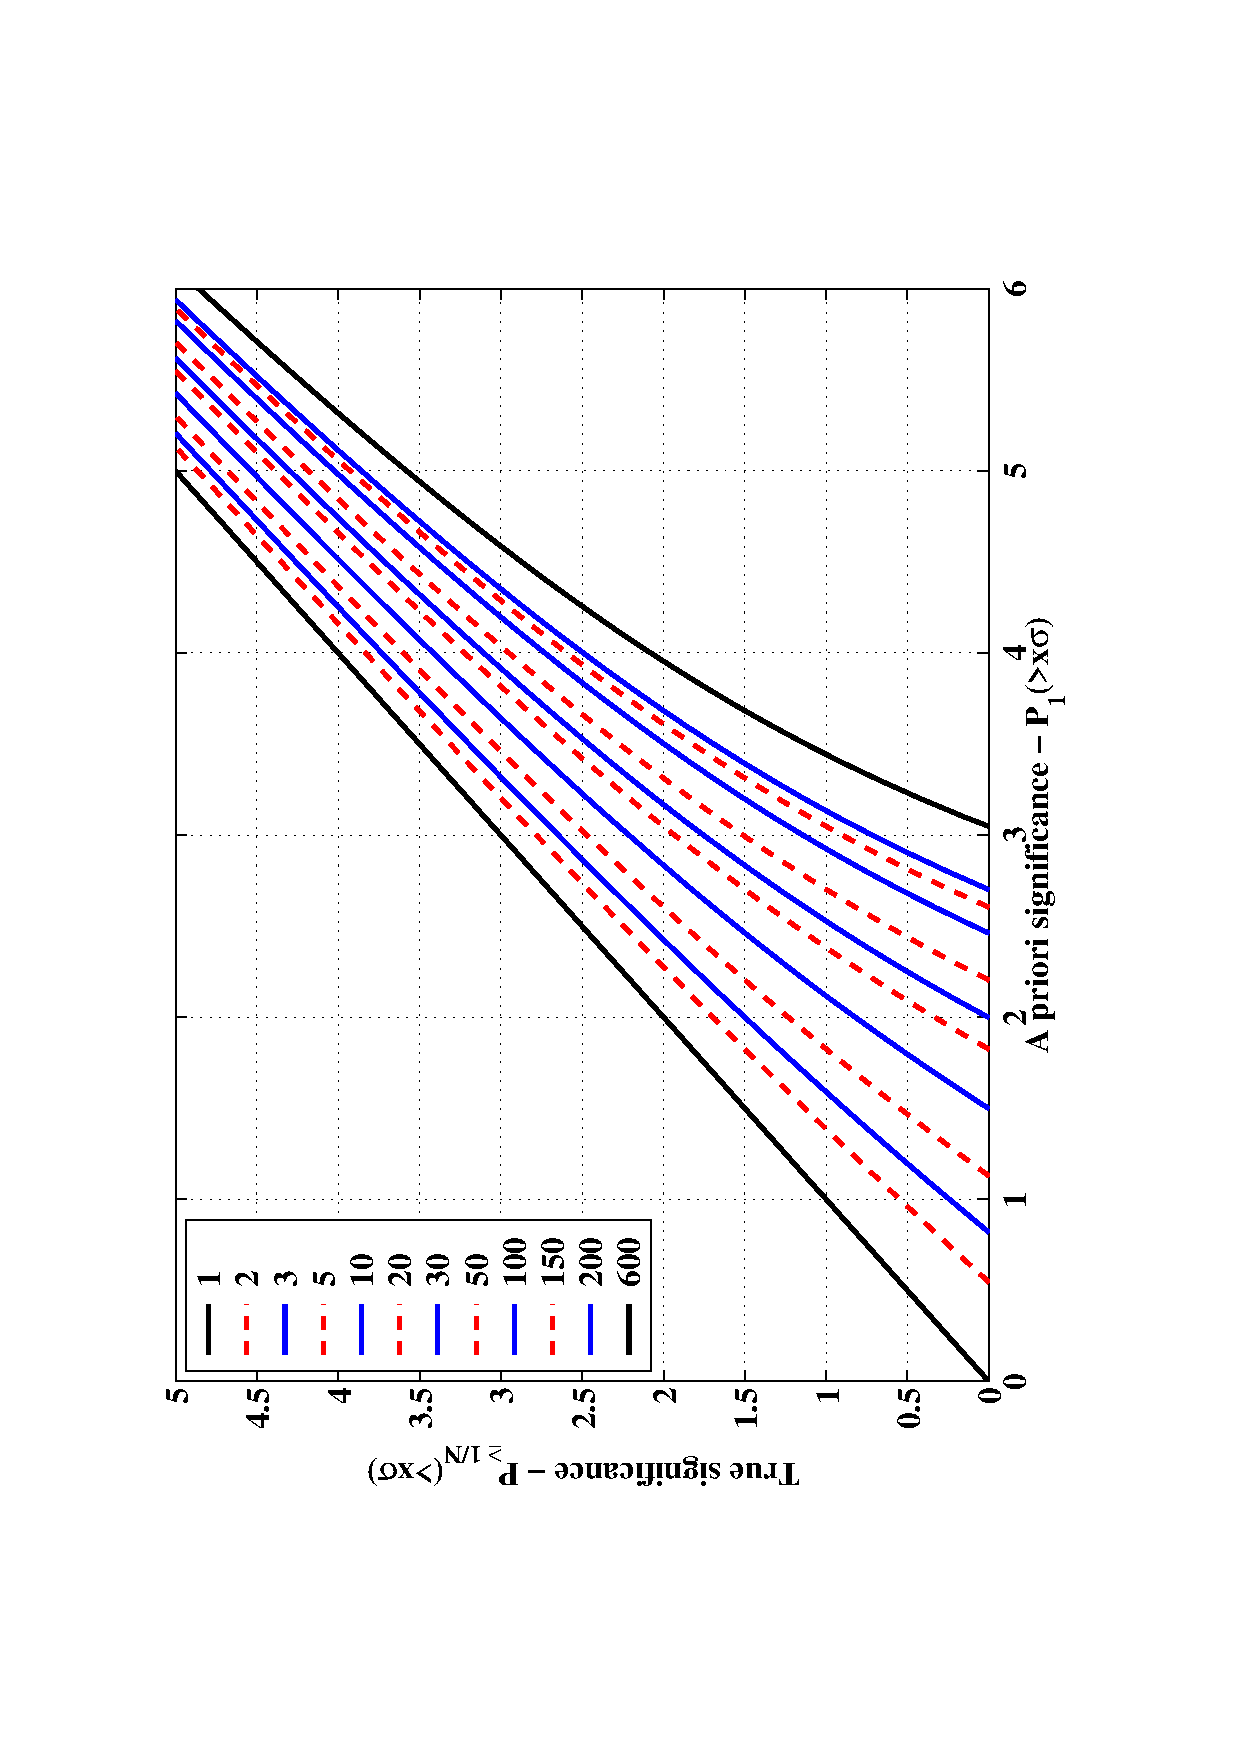
\includegraphics{plots/chap-analysis/sigma.pdf}}}}
\caption{\label{FIG::ANALYSIS::SIGMASIGMA} Probability of at 
least one from $N$ observations giving a result of $>x\sigma$ as 
compared with the probability of a single observation giving the same
result. Curves with increasing $N$, from 1 to 600, go from left to
right.}
\end{figure}

When the location of the source within the field of view is not known
in advance, the null hypothesis must be modified to require that no
source be present anywhere within the field of interest. To reject
this hypothesis a number of independent bins must be calculated and the
``true significance'' of the largest observed excess must be
determined. This ``true significance'' is different from the a priori
significance $\sigma(\vec{r})$ discussed up to this point. The
distribution of the function $\max{\sigma(\vec{r})}$ is not Gaussian
for maps which contain more than one independent bin. Since the term
``significance'' is usually associated with the Gaussian distribution
it is less confusing to refer instead to the probability that the null
hypothesis be true or false.

For a single observation, with Gaussian distribution, the probability
that a result of $>x\sigma$ will be observed, in the absence of a \Gray
source, is given by the error function,
\[P_1(>x\sigma) = \frac{1}{\sqrt{2\pi}}\int_{x}^{\infty}e^{-x'^2/2}\mathrm{d}x' = \{1-\mathrm{erf}(x/\sqrt{2})\}/2.\]
The probability of observing at least one result of $>x\sigma$ in $N$
independent observations, denoted $P_{\geq 1/N}(>x\sigma)$, is
calculated by noting that if such a result is not observed, it must be
the case that \textbf{all} $N$ observations have a result of
$\leq x\sigma$, which is simply the product of $N$ individual
probabilities $P_1(\leq x\sigma)$,
\[P_{\geq 1/N}(>x\sigma) = 1 - \{1-P_1(>x\sigma)\}^N.\]
It is conventional to claim the detection of a source when the null
hypothesis has been rejected at a $>4\sigma$ level
\citep{REF::WEEKES::1999SNOWBIRD}, assuming a Gaussian distribution.
Figure~\ref{FIG::ANALYSIS::SIGMASIGMA} shows how $P_{\geq
1/N}(>x\sigma)$ relates to $P_1(>x\sigma)$. It can be seen from the
figure that a $4\sigma$ Gaussian confidence level (on the y-axis)
corresponds to the probability of detecting at least one
$\sim4.6\sigma$ result with $N=10$ and increases to $\sim5.3\sigma$
for $N=600$.

To relate the curves in figure~\ref{FIG::ANALYSIS::SIGMASIGMA} to the
sky maps generated from real data, an equivalent number of independent
bins must be calculated. The individual bins in the 2-d histogram are
highly correlated, both through the smoothing applied to the image and
the inaccuracy in the reconstruction method. Since the reconstruction
method is difficult to characterize, as are the effects of the edge of
the camera, the number of independent bins in the image is difficult to
calculate. Two estimates can be made, the first by considering the
width of the smoothing and the size of the camera, the second by
fitting for $N$ in the distribution, $P_{\geq 1/N}(>x\sigma)$, of
maximum significances from the dark-field data described above.

For a 2-dimensional Gaussian smoothing function, $g(\vec{r};r_0)=
\exp(-r^2/2r_0^2)$, 50\% of the counts are contained in a region of
radius $r=0.206^\circ$ for $r_0=0.175^\circ$. An estimate of the number
of independent bins can be made for regions of the sky map of various
widths, given by $2R$, by taking the ratio of the area of the region
and the area under the Gaussian. To account for effects at the border
of the region of interest, a border of $0.206^\circ$ can be added, so
\[N \sim \frac{\pi\times(R+0.206^\circ)^2}{\pi\times(0.206^\circ)^2} =
\left(\frac{R}{0.206^\circ}+1\right)^2\]
The estimates for $N$ from this method, with and without the border
effect are shown in table~\ref{TABLE::ANALYSIS::NINDEPENDENT}.

To estimate the number of independent bins from the distribution of
the maximum significance in the dark field data,
\mbox{$\max(\sigma(\vec{r})\;;|\vec{r}|<R)$}, a maximum likelihood
approach is used. For any value of $R$, the size of the region of
interest, analysis of the $240$ dark fields result in a set of maximum
significances, $\{x^{(R)}_i\}=\{\,max(\sigma_i(\vec{r})\;;|\vec{r}|<R)\,\}$.
The likelihood that this set of observations are drawn from the 
probability distribution for $N$ independent Gaussian observations is
given by,
\[L(x^{(R)}_i\,|\,N) = \prod_{i=1}^{240}\left[\frac{\mathrm{d}P_{\geq
1/N}(>x\sigma)}{\mathrm{d}x}\right]_{x=x^{(R)}_i}\] Maximizing the log
likelihood, $\Lambda=\ln L$, gives the best estimate of the number of
independent bins for each region size, $N(R)$. 

Figure~\ref{FIG::ANALYSIS::2DSIGMADISTRIBUTIONS} shows the
experimental distributions for $R=0.38^\circ$, $R=0.55^\circ$ and
$R=1.10^\circ$. The theoretical distribution based on the most likely
value of $N(R)$ is also shown. It can be seen that in the
$R=1.1^\circ$ case, the fit is not particularly good, a result of the
broad tails on the experimental distribution. Also displayed on these
figures is the results of a simple Monte Carlo (MC) simulation of the
smoothing, as described in appendix~\ref{APP::SMOOTHING}. It can be
seen that the likelihood fit to the experimental results matches the
MC distributions well, with the MC distributions being slightly
wider. Figure~\ref{FIG::ANALYSIS::NINDEPENDENTLIKELIHOOD} shows the
function $N(R)$ plotted against the area of the region, $A\propto
R^2$. It can be seen that there is a roughly linear increase of $N$
with $A$, at least for
$R<0.9^\circ$. Table~\ref{TABLE::ANALYSIS::NINDEPENDENT} lists the
values of $N$ for the cases considered above.

\begin{figure}[p!]
%\begin{minipage}{0.33\textwidth}\centerline{$r<0.35^\circ$}\end{minipage}%
%\begin{minipage}{0.33\textwidth}\centerline{$r<0.55^\circ$}\end{minipage}%
%\begin{minipage}{0.33\textwidth}\centerline{$r<1.10^\circ$}\end{minipage}\\
\resizebox*{0.33\textwidth}{!}{\rotatebox{270}{\includegraphics[draft=false]{plots/chap-analysis/dof_exp_like_0_348.pdf}}}%
\resizebox*{0.33\textwidth}{!}{\rotatebox{270}{\includegraphics[draft=false]{plots/chap-analysis/dof_exp_like_0_550.pdf}}}%
\resizebox*{0.33\textwidth}{!}{\rotatebox{270}{\includegraphics[draft=false]{plots/chap-analysis/dof_exp_like_1_100.pdf}}}
\caption{\label{FIG::ANALYSIS::2DSIGMADISTRIBUTIONS} 
Experimental and best-fit distributions for 
$\max(\sigma(\vec{r})\;;|\vec{r}|<R)$, listed
for $R=0.38^\circ$, $R=0.55^\circ$ and $R=1.10^\circ$.}
\end{figure}

\begin{figure}[p!]
\centerline{\resizebox*{0.8\textwidth}{!}{\rotatebox{270}{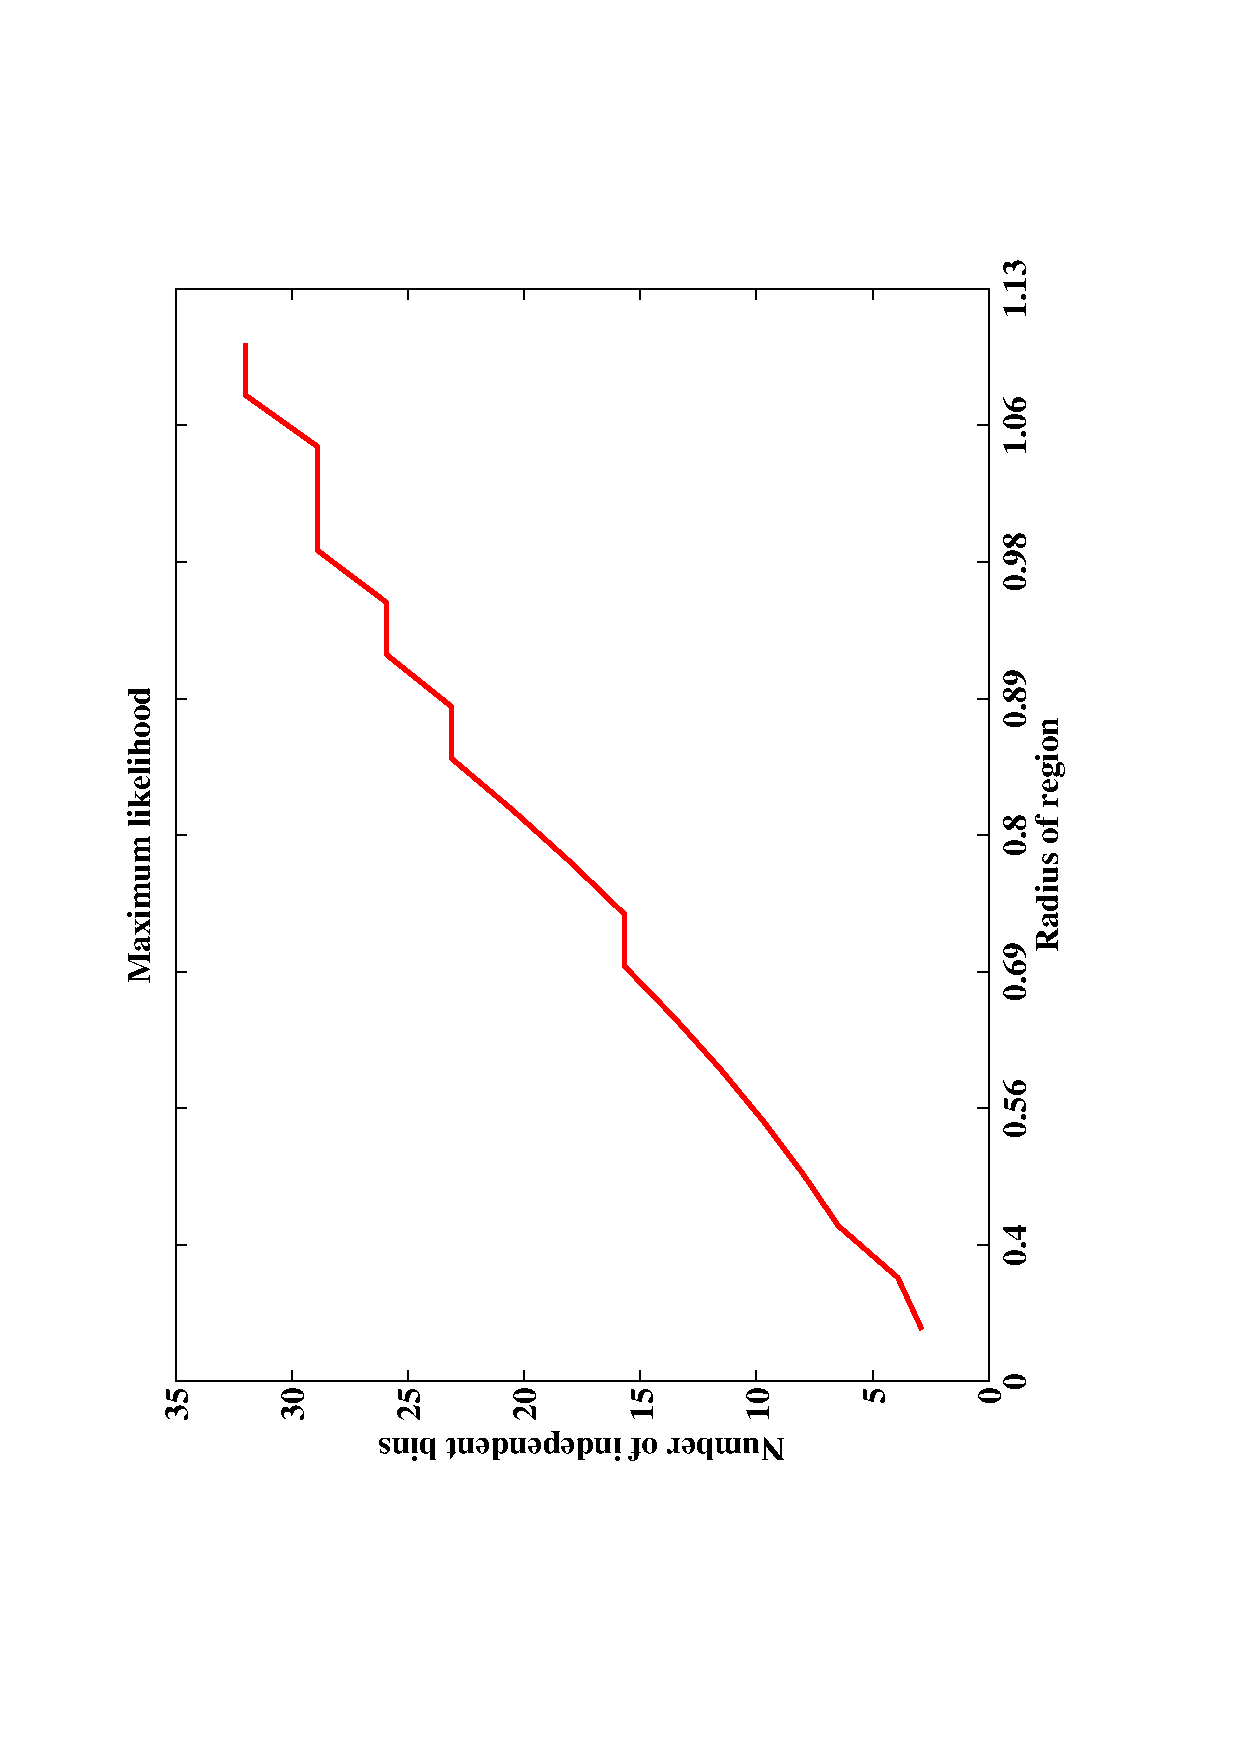
\includegraphics[draft=false]{plots/chap-analysis/dof_like.pdf}}}}
\caption{\label{FIG::ANALYSIS::NINDEPENDENTLIKELIHOOD} 
Maximum likelihood fit for $N(R)$ as a function of $A\propto R^2$.}
\end{figure}

\begin{table}[p]
\caption{\label{TABLE::ANALYSIS::NINDEPENDENT} Estimates 
for the number of independent bins, $N$, present in the region of 
a sky-map of area $\pi R^2$. Three estimates are given, the first 
two express the ratio of the areas of the region and the smoothing 
Gaussian. The final estimate is from a maximum likelihood fit to 
the distribution of maximum significance.}
\centerline{\begin{tabular}{llll}\hline
Method & $R=0.35^\circ$ & $R=0.55^\circ$ & $R=1.1^\circ$ \\\hline
Ratio of areas $(R/0.206)^2$    &  3 &  7 & 29 \\
Ratio of areas $(R/0.206+1)^2$  &  7 & 13 & 40 \\
Maximum likelihood fit          &  4 & 10 & 32 \\\hline
\end{tabular}}
\end{table}

When data from an unidentified EGRET source is analyzed, a map of (a
priori) significance is produced and the EGRET 95\% contour level
overlaid. The area of the region inside the contour can then be used
to calculate an equivalent number of independent bins, using
figure~\ref{FIG::ANALYSIS::NINDEPENDENTLIKELIHOOD}. This value can
then be used to calculate a significance level which is equivalent to
the accepted Gaussian $4\sigma$ confidence level. The map can then be
checked for emission from within the region of interest.

Additionally, the data can be tested to see whether they are
consistent with the null hypothesis that no emission is present in any
of the $18$ candidate fields considered in the survey. The value of
$N$ appropriate is $18\times N(1.1^\circ)\approx 600$, the number of
independent bins in the regions of the sky within $1.1^\circ$ of the
center (the region defined by the edge of the camera) of each $18$
field. A significance level, from
figure~\ref{FIG::ANALYSIS::SIGMASIGMA}, of $\sim5.3\sigma$ is required
to claim the null hypothesis is false with the required confidence.

\section{\Trk\ Analysis}
\label{SEC::ANALYSIS::TRACKING}

For objects whose location is well known, a simpler analysis technique
can be applied. The analysis can take advantage of the \Trk\ mode of
observation, giving twice the amount of on-source data over the \Pairs\
mode. As described above, the analysis takes advantage of the fact
that the candidate source is at the center of the field of view, which
allows events which are not consistent with having originated at the
center of the field of view to be eliminated. The selection is done on
the basis of the \textit{alpha} parameter; a cut of $\alpha<15^\circ$
was been found to be optimal. An estimate of the background is made
from the number of events which are not aligned with the center of the
field of view; those with $20^\circ<\alpha<65^\circ$ are
chosen. Assuming there are $N_{On}$ events with $\alpha<15^\circ$ and
$N_{Off}$ with $20^\circ<\alpha<65^\circ$, the excess counts is given
by,
\begin{equation}\label{EQN::ANALYSIS::TRKEXCESS}
\Delta N = N_\mathrm{On}-\rho\,N_\mathrm{Off}
\end{equation}
The constant $\rho$, termed the ``tracking ratio'', relates the number
of counts with $\alpha<15^\circ$ to the number with
$20^\circ<\alpha<65^\circ$ in the absence of a source. This constant
must be calculated independently with dark field observations. The
significance of the excess is given by propagation of errors,
\begin{equation}\label{EQN::ANALYSIS::TRKSIGMA}
\sigma = \frac{N_\mathrm{On}-\rho\,N_\mathrm{Off}}
{\sqrt{N_\mathrm{On}+\rho^2\,N_\mathrm{Off}}}
\end{equation}

This equation for significance is not completely correct for a number
of reasons. First, the value of $\rho$ calculated from dark field data
has an error associated with it, $\rho\pm\Delta\rho$. The calculation
of significance equation must account for this error, lowering the
significance somewhat. Additionally, as described in
\citet{REF::LIANDMA::1983APJ}, calculation of significance should be
based on a likelihood approach rather than the simple propagation of
errors above, which systematically underestimates the significance (in
the absence of $\Delta\rho$). The corrected equations for significance
are listed in appendix~\ref{APP::LIANDMA}. In practice, the
differences between the calculated values are small, and
equation~\ref{EQN::ANALYSIS::TRKSIGMA} can be employed.


%crab-9900-0.5  7.8  0.0269  0.0035  0.0351
%crab-0001-0.0  13.2  0.0417  0.0032  0.0491
%crab-0001-0.3  11.2  0.0371  0.0033  0.0448
%crab-0001-0.8  7.0  0.0234  0.0034  0.0312
%crab-0001-1.3  5.5  0.0131  0.0024  0.0188
%crab-0102-0.0  7.4  0.0278  0.0038  0.0366
%crab-0102-0.5  8.3  0.0345  0.0042  0.0443
%crab-0102-0.8  4.2  0.0195  0.0046  0.0302
%crab-0203-0.0  16.6  0.0311  0.0019  0.0355
%crab-0203-0.8  7.5  0.0241  0.0032  0.0316
%crab-0203-1.0  1.8  0.0056  0.0031  0.0130
%crab-0203-1.3  4.4  0.0129  0.0030  0.0199


%crab-9900-0.5  4.4  0.0047  0.0011  0.0072
%crab-0001-0.0  7.6  0.0059  0.0008  0.0077
%crab-0001-0.3  7.9  0.0060  0.0008  0.0078
%crab-0001-0.8  3.6  0.0033  0.0009  0.0054
%crab-0001-1.3  2.1  0.0017  0.0009  0.0037
%crab-0102-0.0  3.7  0.0045  0.0012  0.0074
%crab-0102-0.5  4.0  0.0054  0.0014  0.0086
%crab-0102-0.8  3.3  0.0060  0.0018  0.0102
%crab-0203-0.0  8.7  0.0056  0.0006  0.0071
%crab-0203-0.8  4.6  0.0051  0.0012  0.0078
%crab-0203-1.0  1.8  0.0020  0.0011  0.0047
%crab-0203-1.3  2.9  0.0030  0.0013  0.0062

